%\documentclass[german,bachelor]{swsLeipzig}
\documentclass[english,bachelor]{swsLeipzig}
% When you change the language, pdflatex may halt on recompilation.
% Just hit enter to continue and recompile again. This should fix it.

%
% Values
% ------
\ThesisSetTitle{Automatic Identification of Configuration Errors from Stack Overflow}
\ThesisSetKeywords{} % only for PDF meta attributes

\ThesisSetAuthor{Ferris Kleier}
\ThesisSetStudentNumber{3732130}
\ThesisSetDateOfBirth{1}{1}{2000}
\ThesisSetPlaceOfBirth{Ahlen}

\ThesisSetSupervisors{Prof.\ Dr.\ Norbert Siegmund,Prof.\ Dr.\ Unknown Yet}

\ThesisSetSubmissionDate{23}{1}{2024}

%
% Suggested Packages
% ------------------
\usepackage[sort&compress]{natbib}
%   Allows citing in different ways (e.g., only the authors if you use the
%   citation again within a short time).
%
\usepackage{booktabs}
%    For tables ``looking the right way''.
%
%\usepackage{tabularx}
%    Enables tables with columns that automatically fill the page width.
%
%\usepackage[ruled,algochapter]{algorithm2e}
%    A package for pseudo code algorithms.
%
%\usepackage{amsmath}
%    For tabular-style formatting of mathematical environments.
%

%
% Commenting (by your supervisor)
% -------------------------------
\usepackage{xcolor}
\usepackage{graphicx}
\usepackage{tcolorbox}
\usepackage{amsmath}
\usepackage{changepage}
\tcbuselibrary{skins}
\usepackage{soul}
\newcommand{\bscom}[2]{%
  % #1 Original text.
  % #2 Replacement text.
    \st{\scriptsize\,#1}{\color{blue}\scriptsize\,#2}%
  }

% Create links in the pdf document
% Hyperref has some incompatibilities with other packages
% Some other packages must be loaded before, some after hyperref
% Additional options to the hyperref package can be provided in the braces []
\usehyperref[backref] % This will add back references in the bibliography

\begin{document}
\begin{frontmatter}
  \begin{abstract}
    This Bachelor's thesis addresses the critical challenge of identifying configuration errors in software systems, which can lead to problems ranging from poor performance to complete system failure. Due to the increasing complexity of modern systems, errors are often caused by human factors such as lack of expertise and poor communication. Using Stack Overflow, an online developer community, as a data source to classify and analyze configuration errors, this thesis proposes a two-part approach. Firstly, a machine learning model named CM-PaCE is used to recognize patterns in discussions about configuration errors, utilizing the Word2Vec and SVM methods. Secondly, the large language model (LLM) GPT-3.5 by OpenAI is employed to perform similar tasks with a focus on prompt engineering. Both approaches are compared in terms of efficiency, accuracy, and real-world applicability. Subsequently, the LLM is used to analyze datasets for configuration errors, including the type of configuration error, impact of the configuration error, and technology stack involved. This thesis aims to provide a comprehensive overview of configuration errors and their implications. It also aims to investigate the potential applications and limitations of traditional machine learning methods and LLM approaches in this domain.
  \end{abstract}

  \tableofcontents

  %\chapter*{Acknowledgements} % optional
  %I thank the authors of the swsLeipzig template for their excellent work!

  %\listoffigures % optional

  %\listoftables % optional

  %\listofalgorithms % optional
  %    requires package algorithm2e

  % optional: list of symbols/notation (e.g., using the nomencl package)
\end{frontmatter}

\chapter{Introduction}\label{introduction}
In today's fast-paced technological world, the vulnerability of software systems cannot be denied. The main reason
for this is the fact that more complex systems tend to have more bugs. In the configuration process of a system, 
this can lead to various problems such as poor performance or in some cases, complete system failure. \citet{xuzhou:2015} explain that these configuration errors (i.e., misconfigurations), which result from lack of 
expertise or human error in setting up such systems, are an important challenge. They are mistakes made during 
the configuration process of a software system, both during initial setup and to optimize the running system. 
They can cause various problems during runtime, not only in terms of logistics and lost revenue due to downtime, 
but also in terms of security risks. One major example for the impact of configuration errors is the 2021 outage 
of Meta, which resulted from misconfigurations in their network, causing a \$6bn loss in revenue for Meta 
CEO Mark Zuckerberg (\citet{jana:2021}, \citet{guardian:2021}). While these mistakes can be made by anyone involved in the configuration process, 
they are often made by people who are not familiar with the system. Software administrators typically lack 
in-depth knowledge of the systems they manage (\citet{xuzhou:2015}). Another major cause of misconfigurations is the increasing 
complexity that comes with more configuration options. Other reasons for configuration errors may include the 
aforementioned lack of expertise, poor communication, and lack of documentation, among others.

In the context of configuration errors, many developers rely on online resources such as Stack Overflow (SoF) 
to find solutions to their problems. SoF is an online community where users can ask questions about programming 
problems and receive answers from other users. This allows users to find help in resolving issues and share their 
experiences. A dataset of all SoF posts would be extremely useful for extracting knowledge and better analyzing 
different topics, such as configuration errors. Classification models can be used to aid this process, 
since a well-trained model can automatically collect datasets of posts on a specific topic, reducing the manual 
labor required to create such datasets.

According to \citet{yinma:2011}, preventing configuration errors is critical to maintaining the 
functionality and reputation of a system, which leads to our first research question: \textbf{How do different Machine 
Learning Approaches compare to retrieve Stack Overflow posts about configuration errors?} The goal is to develop 
an approach that uses machine learning algorithms to automatically identify Stack Overflow posts about 
configuration errors. On the one hand, we will manually develop a machine learning model. The model of this 
first approach will be trained to recognize patterns of discussions about configuration errors in order to 
retrieve a set of posts from the platform. In the second approach, we will use the large language model gpt3.5-turbo, for which we will configure the model to do the same as in the first approach. We will use different 
prompting methods to find the best method for our task. After both models satisfy the expectations, we will 
compare both approaches in terms of efficiency, accuracy of results and applicability in real scenarios. Finding 
the best method to retrieve posts from Stack Overflow leads to the second research question of this thesis: 
\textbf{How do LLMs help to analyze retrieved datasets?} In this part, we will use the large language model gpt3.5-turbo to analyze a retrieved dataset 
of posts in terms of misconfigurations, such as the category of misconfiguration or the impact on the system.

To achieve our research goal, we will use a data dump of Stack Overflow posts (\citet{stackexchange:2023}), which includes anonymized 
usernames, tags, and other relevant meta-information. From there, we will manually select posts that contain 
misconfigurations and not, using defined criterions. Using the Python programming language and the Word2Vec 
method, we will extract terms from the posts and detect those related to misconfigurations using the SVM 
supervised learning method. As a result, we will train a machine learning model to recognize typical 
misconfigurations using the set of labeled posts, the training set, and evaluate the model using a separate 
test set. This serves as the first approach for the first research question. The second approach uses the 
gpt3.5-turbo model, for which we will use the API to build a model that fits our expectations. 
We expect this model to generate natural and coherent responses that can answer the question of whether a post 
is about configuration errors or not. We also expect the model to be able to handle different levels of user 
expertise. In this way, we can easily iterate over a set of posts and significantly reduce the training process 
to just prompt engineering. We then compare the two approaches on various aspects and evaluate which approach 
works best to retrieve a desired set of posts about configuration errors. For the second research question, 
we use the gpt3.5-turbo model to analyze a previously retrieved set of posts about configuration errors on various 
characteristics, such as their technology stack, the cause of the error, and  the type of the error. This allows 
for a deeper understanding of the work and shows the applicability of both approaches.

To structure this thesis, we first explain the problem of configuration errors to further solidify our motivation. 
Then we discuss the idea behind using Stack Overflow posts and where we got the data dump from. For the methodology, 
we explain on which features we trained the first model and how we trained it using all the necessary tools in 
the Python programming language. To illustrate the second approach, we talk about the API that powers GPT-3.5, 
how we implemented it for use, and all the necessary processes like writing the prompts. After that we use 
the gpt3.5-turbo model to analyze a set of posts and show the applicability. We then show the results of both experiments, 
including accuracy, examples of use cases, a discussion of limitations, and what problems we encountered that 
are still limiting. Next, we evaluate the results in the Discussion chapter, discussing both classification 
approaches about the differences between them, how they compare to each other, and their significance. Finally, we 
evaluate the third experiment and provide ideas for future research in this area.\\

In order to facilitate a comprehensive understanding of the practical applications and methodologies discussed in this thesis, 
readers are encouraged to visit our repository on \citeauthor{repo}, where the complete code and additional resources are available for review.

\chapter{Background}\label{background}
In this section, we provide some definitions to understand the broader topic of software configuration errors. 
We also describe the concept of configurations, further explain configuration errors and why it is important to 
better understand them.

\section{System Configuration}\label{system_configuration}
Configuration in software systems refers to system management operations, such as determining and setting the values 
of various system parameters. \citet{xuzhou:2015} define ``configuration to be the operations that determine 
the values of system settings. The goal of configuration is to transform the system from an unsatisfying state to the 
intended state by changing the settings''. Transforming a system from an unsatisfying state to an intended state 
describes the necessary changes in system settings to increase system performance or solve unintended problems. 
For example, suppose we have a theoretical application A (the system) that is observed to perform poorly, resulting 
in an unsatisfying state of the system. Upon investigation, the problem turns out to be insufficient RAM allocation 
for the application. By increasing the RAM allocation for the system in the settings, and thus changing its values, 
we have transformed the system to an intended state by configuration. 

Configuration can be divided into two types: 
domain-specific configuration and technical configuration (\citet{siegmund:2020}). Domain-specific configuration  is a way of customizing 
a software system to meet the needs of end users. It involves tailoring the system to the user's requirements and 
often involves feature toggles that can be changed at runtime. Technical configuration is further divided into 
infrastructure configuration and development configuration. Infrastructure configuration ``refers to adjusting a 
software system to the underlying hardware and software [\ldots]'' (\citet{siegmund:2020}). Development configuration includes setting up 
development and build tools, the build and test process, and automated deployment processes.

We can think of a configuration as a set of underlying settings of a system that determine various aspects such as 
functionality, performance, reliability, or security. These settings can include hardware configurations like RAM 
allocation or database connection settings, where a configuration specifies the parameters used to establish and 
maintain the connection between a program and the database server, such as host, port, username, password, and 
database name. Other examples of configurations include various security settings such as timeout duration, encryption 
keys, and firewall rules (\citet{atlassian:2023}). For firewall rules, a configuration determines which ports, protocols, and addresses 
are allowed or denied, and how network activity is monitored and logged. Modern cloud software systems, such as 
Amazon Web Services (AWS) or Microsoft Azure, use configuration settings to customize the behavior and performance 
of their applications and resources.

Configuration settings can be defined as key-value pairs, environment variables, files, or scripts that specify 
various parameters. These are typically stored in configuration files, usually in JSON or YAML format. \citet{huang:2017} define configuration files as ``a file that stores application state that is neither task-dependent nor 
time-dependent, and whose contents may thus affect an application's availability or performance over a period of 
time and across a number of tasks'' (\citet{huang:2017}). The advantage is that configuration settings are stored in a single file, 
or in different configuration files for different modules. As with all structured files, it is important to test 
them and make sure they work. In this way, we can customize a system by simply accessing the configuration file, 
either directly or through a user interface, and changing certain values.

System configurations are typically managed by system administrators and developers who set up the system, configure 
the system and hardware, manage user accounts, perform performance tuning, or analyze system logs (\citet{wikimedia:2022}). According to 
Siegmund et al. (2020) ``a developer may be responsible for configuring the environment of the software system (e.g., 
using Docker) and the infrastructure (e.g., database connection, microservice deployment, resource management, and 
network communication)'' (\citet{siegmund:2020}). As a result, system administrators and developers are highly susceptible to human error. 
In addition to these tasks, system administrators are responsible for ``system maintenance and configuration, such as 
installing and troubleshooting hardware and software'' (\citet{hanna:2021}), which essentially means that they are obligated to 
respond to system failures or configuration errors that occur either in their local system or in the cloud systems 
on which they operate. Software developers, on the other hand, are highly responsible for testing their software 
to prevent errors caused by unexpected behavior. The important issue of configuration errors is discussed in the 
following section.

\section{Configuration Errors}\label{configuration_errors}
Configuration errors are configurations that, due to improper settings, transform a software system from a functional 
state to an unsatisfying state or, in the worst case, to a total system failure. This can be noticed by various 
symptoms such as slow performance, security vulnerabilities or, according to \citet{zhang:2013}, incorrect 
output or unexpected termination. As proposed by \citet{yinma:2011}, there are three categories of 
configuration errors:

\begin{itemize}
  \item \textbf{Parameter Misconfigurations:} This type of configuration error can result from illegal 
  misconfigurations that violate a system's rules of format, syntax, or semantics. Essentially, this means that 
  a configuration is not allowed because there is no option for which the system is prepared to operate on. Some 
  examples include using a comma instead of a semicolon for key-value pairs in a JSON file, mixing data types 
  like string and integer in functions, or mixing tabs and spaces for indentation in a YAML file, which can lead 
  to serious problems in cloud systems when such a YAML file is used to configure Infrastructure as Code (IaC). 
  There are also legal misconfigurations that are allowed but do not provide the desired functionality. An example 
  would be setting the wrong time zone in a server. This can lead to problems such as incorrect timestamps or 
  automation inconsistencies.

  \item \textbf{Software Incompatibility:} These can be caused by incompatible components or versions and can 
  lead to misconfigurations after a system is installed, such as software designed for a 64-bit processor that 
  does not run properly on a 32-bit processor. Another is a configuration that works for the system being used, 
  but causes problems in future generations due to hardware changes or differences in software versions, leading 
  to system instability, crashes, and errors. Other scenarios include multiple applications that share resources 
  but have different requirements for those resources.

  \item \textbf{Component Misconfiguration:} \citet{yinma:2011} define these as ``Configuration errors 
  that are neither parameter mistakes nor compatibility problems''. This term includes `missing components', 
  `placement of files', `file format', `insufficient resources', and `stale data'. For missing components, a web 
  server may not work if certain libraries are missing. File placement covers all cases where files or dependencies 
  are either in the wrong directory or have different names than referenced. The same goes for incorrect file 
  format, where the system may not work because the configuration file has incorrect syntax, such as missing 
  brackets. Inadequate resources refers to low memory allocation or missing disk space. Finally, stale data refers 
  to outdated data, such as old configuration files that technically work but are rejected by the firewall.
\end{itemize}

\citet{xuzhou:2015} characterized the two main causes of configuration errors, which include system errors and 
human errors. Configuration errors caused by system errors include failed uninstallation of applications, software 
bugs, corrupted registries, and so on. These causes can interfere with the desired function of a system and create 
conflicts or inconsistencies in the configuration settings. Failed application uninstallations can leave behind 
unwanted files or registry entries that can cause configuration errors. For example, an application that is not 
uninstalled properly may try to access some resources that are no longer available or compatible with the current 
configuration. This can result in errors such as corrupted registries, invalid shortcuts, or broken dependencies. 
Software bugs that are configuration errors are defects or flaws in the code or design of a software program that 
can cause it to behave unexpectedly or incorrectly and damage a configuration. A corrupted registry, caused by 
various reasons like malware or disk failure, can cause configuration errors by preventing the system from reading 
or writing the correct values for the configuration settings.

In summary, configuration errors caused by system 
errors are difficult to prevent due to their various causes. Misconfigurations caused by human error, on the other 
hand, are caused by misspellings, hitting the wrong line when checking settings or editing configuration files, 
or simply making the wrong decision in a large set of options. There are several ways to prevent human errors, 
including automation tools such as scripts to check for inconsistencies caused by misspelling. Reviewing and checking 
logs is also a common way to track these types of errors, and it is generally a good practice to double check after 
the setup process to account for human error. It is also important to prepare and train system administrators for 
their area of responsibility. Finally, the complexity of software configurations creates exponentially more room 
for error due to the growing permutations with more options.

\section{Tackling Configuration Errors}\label{tackling_configuration_errors}
Existing approaches to counter misconfigurations include an idea by \citet{rabkin:2011} to support users with error
 messages in the software library called Hadoop. Apache Hadoop is used in big data processing for parallel processing on large data sets. It enables applications to run on systems with thousands of nodes and petabytes of data, allowing for search engines or other systems to construct large indexes. When a user encounters an error message, their system ``points them to a configuration option that, if changed, will make the error go away'' (\citet{rabkin:2011}). This idea is barely suitable for larger software systems, since, as was already indicated, the growing complexity of software configurations and therefore a slower response rate for this approach is to be expected, leading to slower runtimes to find every possible error. Another approach was proposed by \citet{yinma:2011} to build `configuration-free systems`. The idea behind this term is to restrict configuration options and automate a wide variety of tasks.

In a study conducted by \citet{siegmund:2020}, interviewees proposed further best practices to avoid configuration 
errors, including explicit modeling of options, moving run-time configuration to build-time configuration, and simplifying configuration. Explicit modeling of options refers to documenting the intent of configuration options and discussing if an option is necessary or not. To achieve this approach, they propose a ``meta-configuration'', which consists of validation, management, and finding relations between configuration values, their names, and data types. The move from run-time configuration to build-time configuration aims to validate software as soon as possible during the building of software and avoid redundant time to fix errors after deployment and development. Finally, simplifying configuration involves two ways to help users work with deployed configurations. In one respect, users are guided through the configuration process. This helps the user to better understand what configuration options make sense to be configured. The idea is a practice called ``Convention over Configuration''. The interviewees describe this practice for a stakeholder who ``provides a feasible pre-configuration that is hidden from the user, avoiding the need to dig deep into configuration files. The stakeholder (e.g., ops engineer) who then owns the configuration can diverge from the standard values to adapt the system to their needs'' (\citet{siegmund:2020}).

There are three more ideas to address configuration errors. The first is static analysis. It aims to utilize automation 
and configuration management tools to ensure consistency and accuracy in configurations. This includes checking for syntax errors, semantic errors, and inconsistencies, all through automation tools to find errors where data is not used correctly or where data is used in an unexpected way (\citet{dong:2013}, \citet{johnson:2011}). The second approach is dynamic analysis, which monitors the system while it is running to detect configuration errors. This differs to static analysis insofar as the detection is prior to the running of the software (\citet{bellairs:2023}). The goal is to implement continuous monitoring mechanisms that detect and report configuration errors (\citet{atta:2010}). Finally, the third approach is to perform regular testing and validation of configurations to identify errors or vulnerabilities (\citet{owasp:2023}). This process includes reviewing, approving, and testing changes before they are deployed and used. A good practice for this third approach is to conduct penetration testing and vulnerability assessments to resolve configuration-related problems. Overall, there have already been many different approaches and ideas to address configuration errors and help users manage them.

\section{Word2Vec \& SVM}\label{word2vec_svm}
We decided to use Word2Vec for the feature extraction part of our first approach, following an analysis by \citet{tian:2020} on methods to detect architecture smell discussions on Stack Overflow, which resulted in Word2Vec having the highest accuracy and F1-score in combination with classification methods. For the classification method, we came to the conclusion that the Support Vector Machine (SVM) method best suits our work, following their work as well. The combination of Word2Vec and SVM, according to their study, represented the best overall accuracy and F1-Score, directly followed by the Term Frequency-Inverse Document Frequency (TF-IDF) method in combination with SVM.

\subsubsection{Word2Vec}
Word2Vec is a machine learning method used for several tasks like natural language processing (NLP) or information 
retrieval. It was developed by \citet{mikolov:2013}. It learns high-quality word embeddings as vector representations of words from a corpus of text. These vector representations represent the semantic and syntactic relationships between the words in a corpus. The two main models of Word2Vec are Continuous Bag-of-Words (CBoW) and Skip-Gram (\citet{tian:2020}). Continuous Bag-of-Words predicts the current word from its surrounding words. Skip-Gram predicts the surrounding words from the given, current word. For this work, we decided to use the Skip-Gram model because of popularity and because it is better suited to capture the semantic relationships between words. Word2Vec is typically used to train a neural network on a set of documents. After training the model, it outputs a vector representation of each word in the corpus \citet{li:2019}. In this way, Word2vec is useful for information retrieval tasks by taking these vector representations and comparing them to other documents to find similarities. For our purpose, we will use the Skip-Gram approach, since context is more important than frequency. If a post contains code with many repeating words, this could lead to bias in the CBoW approach.

\subsubsection{Support Vector Machine}
A support vector machine (SVM) is a supervised learning method used for linear classification and regression, whereby it 
is preferred for classification tasks. The advantages of SVMs include the effectiveness in high dimensional spaces and memory efficiency, while a disadvantage is that SVMs offer no direct probabilities, which are rather calculated using five-fold cross-validation (\citeauthor{scikit:nd}). In itself, SVMs can only perform dichotomic classification, although there exist some approaches for multi-class problems (\citet{franc:2002}). The basic approach of an SVM for classification is to find a hyper-plane that separates data into two classes. This is done by plotting the data items from the dataset into an n-dimensional space, where n is the number of features we extracted earlier using Word2Vec. After that, the algorithm finds the optimal hyperplane to separate the data (\citet{geeks:2023}). Ultimately, a trained SVM model is useful for tasks such as finding documents that are relevant to a specific topic, which ideally serves our purpose to classify Stack Overflow posts according to their talk about configuration errors.

\section{LLM \& Prompt Engineering}
\subsubsection{GPT-3.5}
GPT-3.5 is a natural language processing (NLP) large language model (LLM) capable of generating human-like answers 
generally in the form of chat-like conversations using queries (also called prompts) (\citet{bahrini:2023}). Recently, it has become a popular and very powerful tool to create generative text-based content for different purposes such as education, translation, medicine, or code generation (\citet{liu:2023}). GPT stands for Generative Pre-trained Transformer, meaning that it can generate new data and is pre-trained to work on the given data. ``Transformer'' refers to a neural network algorithm optimized to learn relationships between data (\citet{perrigo:2023}). The GPT model is trained on a large set of data originating from websites, open source code, or documents in PDF format (\citet{bahrini:2023}).

A major benefit of GPT-3.5 is the ability to define domain-specific knowledge from the prompt, allowing for fine-tuning 
and directing the AI to respond in respect to a role it was assigned. In this study, we make requests to the API of \citeauthor{openai:2023} using the gpt3.5-turbo model to classify if SoF posts are related to configuration errors, and if so, extract information about these configuration errors if available such as the involved technologies, type, cause, and solution.

\subsubsection{Prompt Engineering}\label{sec:pe}
The use of GPT-3.5 for our task substantially relies on the process of prompt engineering. According to \citet{white:2023} ``a prompt sets the context for the conversation and tells the LLM what information is important and what the desired output form and content should be''. The general process of prompt engineering includes identifying the task, choosing the right language, providing context, and experimenting to get the desired output. That way we can increase the probability that the LLM will produce a desired answer with proper context (\citet{reynolds:2021}). There are three types of prompt engineering which we will use to approach the task in different ways.

\begin{itemize}
  \item \textbf{Zero-Shot Prompting:} The Zero-Shot Learning approach for prompt engineering of LLMs (\citet{luo:2023}, \citet{wei:2021}) works by 
  performing tasks without any prior training on the task. This is done by providing the LLM with a prompt that describes the task in natural language. Zero-Shot Learning is considered to have flaws, since the LLM is not optimized for domain-specific knowledge or may have bias, hence needs instruction tuning to produce desired outputs more correctly (\citet{wei:2021}). Zero-Shot Learning in itself is a quite powerful technique if the LLM is trained properly, and therefore offers a use case for users who want to use it for general tasks without having to invest the time and resources to train the LLM on a dataset for each task.

  \item \textbf{Few-Shot Prompting:} This type of prompt engineering, also called in-context learning, makes use of 
  examples provided to the LLM that will create some context for generating content (\citet{brown:2020}). By providing a set of examples on what a desired output would look like, the LLM can be pre-trained to learn new tasks (\citet{touvron:2023}). On the one hand, few-shot learning offers a significant reduction for task-specific data to be trained on and it is less likely to learn an overly narrow distribution from the dataset. On the other hand, Few-Shot Learning showed worse results than other fine-tuned models (\citet{brown:2020}). To sum it up, this method learns on a set of examples to rapidly adapt to new tasks.

  \item \textbf{Chain-of-Thought Prompting:} In this type, chains of thought demonstrations are presented to the LLM as 
  examples for generating a desired output (\citet{wei:2022}). A chain of thought refers to a set of reasoning steps that result in an output, helping the LLM to understand concepts that will then be applied to generate an answer. These reasoning steps are generally in the form of step-by-step answer examples, resulting in complex decision capabilities (\citet{kojima:2022}). There are two main variants of Chain-of-Thought Learning, Zero-Shot Chain-of-Thought learning and Automatic Chain-of-Thought learning. Zero-Shot Chain-of-Thought learning helps the LLM to come up with chains of thoughts by putting `Let us think step by step' before the output that is to be generated (\citet{kojima:2022}). Automatic Chain-of-Thought learning works similar to Zero-Shot Chain-of-Thought learning, but expands the manual pre-training by creating examples using the `Let's think step by step' method. This way the LLM achieves context on how `Let's think step by step' works and in what way it will apply it to the generated output (\citet{zhang:2022}). Overall, Chain-of-Thought learning improves the ability of an LLM to generate content using reasoning methods. On the one hand this is useful to put context on the pre-training process that an LLM can later use to follow specific steps, while on the other hand this type of prompt engineering is more expensive in computing power and needs sophisticated manual labor.
\end{itemize}

Prompt engineering is an important process when working with LLMs like gpt3.5-turbo, because the results heavily depend 
on the domain knowledge of the model, which in turn depends on provided information that it can construct and work on. This intercedes to improve the performance of LLMs, making them more usable for tasks such as our retrieval approach. However, since prompt engineering is a relatively new field, there are some issues to pay attention to. For one, through proper prompt engineering, the LLM may be able to generate content that it would not normally generate. This process is called `Jailbreaking' and can be abused by malicious users to generate harmful answers, like writing code to program a virus (\citet{liujailbreaking:2023}). `Hallucination' is another unintended behavior of LLMs, where the model generates unrelated or unreal content for prompts that did not intentionally aim to achieve this. In the end, prompt engineering is a complex task that can be used to leverage the full potential from LLMs.

\chapter{Related Work}\label{related_work}
In this Section we will introduce some works that capture ideas related to our approach on tackling configuration errors as well as new ideas in the field of prompt engineering.

\subsubsection{Challenges in Docker Development: A Large-scale Study Using Stack Overflow}
This study by \citet{haque:2020} presents a large-scale empirical study that identifies practitioners' perspectives on Docker technology by mining Stack Overflow (SoF) posts. The authors find that most developers use SoF to ask questions about a wide range of Docker topics, including framework development, application deployment, continuous integration, web server configuration, and more. The team used a tag search to collect a dataset of Docker-related posts, searching for the tag "docker" and collecting a large number of documents for analysis. Most of the posts fall into the application development, configuration, and networking categories. They found that the posts related to status monitoring, data transfer, and user authentication are more popular among developers compared to the other topics. Specifically, developers face challenges with Web browser issues, network errors, and memory management. In addition, there is a lack of experts in this area. In the context of our work, this study provided a different perspective on collecting Stack Overflow posts and a way to see how developers ask questions about configuration bugs. In this way, we can better understand how to analyze a set of retrieved posts, while looking at the challenge of manually collecting posts from a different perspective.

\subsubsection{Dimensions of software configuration: on the configuration context in modern software development}
\citet{siegmund:2020} conducted qualitative research by interviewing various developers from different backgrounds, 
including developers and a cloud foundation architect. The paper provides a comprehensive overview of the different dimensions of software configuration, starting with a definition of configurations and different interpretations of it. Following the evaluation of the interviews, the authors identified eight dimensions of software configuration, including Type, Artifact, Complexity, and Intent. For example, the type of configuration can refer to the various types of artifacts that are configured, such as software, hardware, or infrastructure. It may also refer to several configuration options for these artifacts, including manual and automatic configuration. Next, the paper proposes terminology and context for future research, helping them to better understand and react to configuration errors. The authors continue with best practices to react to configuration errors and the significance of performance engineering, as well as some threats to validity, with the low number of interviewees being the main issue of validity. Finally, the authors conclude that their model contributes to future research, closing with further lessons on configuration such as ``Configuration is code, but often without a well-defined grammar and type system.'' (\citet{siegmund:2020}). In summary, this paper helped to better understand the realm of configuration errors, categorize various features of configuration errors, and learn about best practices as well as ideas for application, including performance optimization. In context to our work, these insights helped to facilitate an understanding of configuration errors and how developers think about them. While this work focussed on the definition and different categories of configuration, these objective thoughts by developers still play a large role when analyzing Stack Overflow posts, which are written by developers as well. That way we can further understand how people ask questions about configuration errors, how to assess their domain knowledge about a topic, and what important features may result from their problem.

\subsubsection{Systems approaches to tackling configuration errors}
This paper by \citet{xuzhou:2015} gives a good introduction to the topic of configuration errors and introduces some 
state-of-the-art approaches to tackle them. They propose some ideas such as building configuration-free systems. This approach tries to eliminate configurations by automatizing them to reduce the complexity of system configurations and help the user react more rationally on a smaller set of options. Even though this idea sounds preferable at first, the authors argue that there should be a balance between too much configuration and complete automation. As we already talked about this in the ``tackling configuration errors'' section, this approach highly limits flexibility for users to adapt the system to different events. Another idea that was brought up by the authors proposes to reuse configuration solutions where a working solution for a particular use case is provided that can be edited for system-specific parameters. With this approach, we can reduce misconfigurations since we only reuse configurations that already worked. However, that way we can still encounter problems, either by changing dependencies that make reusable configurations not working anymore, or by unpredicted scenarios that need new configurations to be set up.  While this paper focuses on direct approaches to reduce the rate of misconfigurations, our approach acts more like an analyzation tool for configuration errors and better understanding them. Nevertheless, it is important to mention the insights from this paper, such as the balance between too much configuration and full automatization.

\subsubsection{Automatic Identification of Architecture Smell Discussions from Stack Overflow}
This paper by \citet{tian:2020} introduces ``an approach to automatically identify [Architecture Smell (AS)]-related posts from Stack Overflow by using machine learning algorithms''. The authors evaluated ``the performance of 12 classifiers based on 3 feature extraction techniques and 4 classification algorithms with a created dataset of SoF posts''. In their work, they manually labeled a total of 395 posts to either contain AS-related content or not and trained their different machine learning models on this set. That way, they can easily find related posts. For the results, they found that ``(1) the TF-IDF [Term Frequency - Inverse Document Frequency] technique performs best when extracting text features to identify ASs; (2) the SVM [Support Vector Machine] based classifier achieves the best overall performance [\ldots] of automatic AS discussions classification; and (3) the SVM algorithm with Word2Vec outperforms the other combinations when automatically identifying AS-related posts''. This work sets up a similar appeal to our work. Just like their approach, our model will be trained to find content-related posts on SoF to support users in finding relevant answers as well. From the insight of their research, we decided to choose Word2Vec in combination with the SVM algorithm to extract and classify posts from our dataset in the first approach. As we already mentioned, we are also researching the usability of a second approach using LLMs. This paper additionally explained a significant amount of techniques to gather SoF posts and analyze the model's performance. This will help us decide on how to collect the posts and label them in accordance to their content. For the criterions to label the posts, we also used the ideas proposed in this paper and modified them to fit our domain of work.

\subsubsection{Automated Diagnosis of Software Configuration Errors}
In this paper, \citet{zhang:2013} propose a technique with a proper tool implementation called ConfDiagnoser 
``to identify the root cause of a configuration error --- a single configuration option that can be changed to produce desired behavior''. This approach uses static analysis, dynamic profiling, and statistical analysis to automate a traceback to the underlying root problem. That way configuration errors can be traced back according to the execution of commands from the error to the initial beginning in the system, and evaluate which configuration changes resolve the issue. Their major findings include that their technique ``is effective in diagnosing both crashing and non-crashing configuration errors with a small profile database''. However, this approach is also not suited for bigger complexity, since we already talked about the fact that diagnosers will have longer runtimes and problems finding errors with more configuration options being available. Nonetheless, we believe that our technique is a great addition to the proposed future work by the authors, which seeks to fix configuration errors. Using our approach, the users can continue to further analyze the configuration errors by the root cause they found with ConfDiagnoser.

\subsubsection{Predicting Performance of Software Configurations: There is no Silver Bullet}
Predicting the performance of software configurations is a difficult topic which this paper aims to explore. \citet{grebhahn:2019} argue that there is no ``silver bullet'' that can be utilized to predict the performance of software configurations with high accuracy. Rather, the authors propose a combination of various machine learning approaches to improve the accuracy for performance prediction. In order to compare the mean prediction accuracy when predicting the performance across all configurations, the authors took into account six machine-learning techniques, 18 sampling strategies, and six subject software systems (\citet{grebhahn:2019}). A dataset of 1,000 software configurations is used in the study to compare the performance of several machine learning techniques, including linear regression, support vector machine, decision trees, as well as a combination of different techniques. The learning technique and sample plan both had a significant impact on prediction accuracy, the authors discovered. They also noted that in most situations, some learning techniques, such as random forests, perform better than others, while the combination of different techniques achieved the best accuracy for prediction software configuration performance. Additionally, because the prediction accuracy is highly dependent on the subject system, there is no learning technique and sampling strategy combination that is consistently the best option when balancing accuracy and measurement overhead. Overall, this study helps to recall that it is important for our approach to consider the specific factors that are relevant to the particular system that is being studied. This will get important when we discuss the application of our approach to analyze configuration errors to better understand them. Finally, the fact that machine learning techniques cannot properly replace sound engineering practices further calls for a method to retrieve information about configuration errors to tackle them in advance.

\subsubsection{Finetuned Language Models Are Zero-Shot Learners}
In this paper, \citet{wei:2021} investigate a straightforward technique for enhancing the zero-shot learning 
capabilities of language models. They work with several prompt engineering methods we presented earlier, showing that instruction tuning significantly improves the capabilities of zero-shot learning on unseen tasks. These tasks include natural language inference, translation, and question answering. The goal of instruction tuning is to teach the language model how to follow instructions. Their methods include taking ``a 137B parameter pretrained language model and instruction tune it on over 60 NLP datasets verbalized via natural language instruction templates'' (\citet{wei:2021}). Their instruction-tuned model, called FLAN, is then evaluated on unseen task types, significantly improving the performance without fine-tuning as well as surpassing the zero-shot and the few-shot GPT-3 model. This is possible because fine-tuned language models are able to learn the relationships between various concepts, even if they have never seen those concepts together before. Furthermore, the number of fine-tuning datasets, model scale, and natural language instructions are an important factor for successful instruction tuning. Overall, the paper provides a promising new approach to zero-shot learning with the potential to be used to learn new tasks, without the need for extensive training data. This helps to better approach upcoming challenges with zero-shot prompting and expands the number of methods to use.

\subsubsection{Prompt Programming for Large Language Models: Beyond the Few-Shot Paradigm}
This work by \citet{reynolds:2021} investigates the few-shot paradigm regarding its performance. The authors 
propose methods for prompt programming, a technique where LLMs solve a wide range of tasks by providing them with a short, well constructed prompt. Their methods include constructing prompts that cause a language model to ``break a problem into components before producing a verdict'' (\citet{reynolds:2021}), followed by the concept of metaprompt programming, which makes the language model write a well-constructed prompt by itself to solve a task. The authors propose future research on this concept of metaprompt programming, stating that ``We are entering a new paradigm of human-computer interaction in which anyone who is fluent in natural language can be a programmer'' (\citet{reynolds:2021}). In summary, this work presents a new method for prompt programming that is more powerful than traditional methods, making it useful for our research by using the breaking-down method of a language model as one method for the posts we want to categorize.

\chapter{Methodology}\label{methodology}
In this section, we will discuss the overall methodology of our study and further explain the importance of our research 
questions, `\textbf{How do different Machine 
Learning Approaches compare to retrieve Stack Overflow posts about configuration errors?}' and `\textbf{How do LLMs help to analyze retrieved datasets?}'. The first part focuses on collecting the necessary data from Stack Overflow using various criteria and keywords. The next part presents the methodology for our first approach, which is a traditional machine learning technique using Word2Vec and SVM. Then we will present the methodology for the second approach, which uses the LLM gpt3.5-turbo by OpenAI. After this, we will address the second research question in the third experimental setup, using a retrieved set of posts, which will be used to analyze configuration errors using the gpt3.5-turbo model as the performing LLM. Figure \ref{fig:figure41}--\ref{fig:figure44} illustrate our methodology for the dataset creation, first experiment, second experiment, and third experiment.

\begin{figure}[h]
  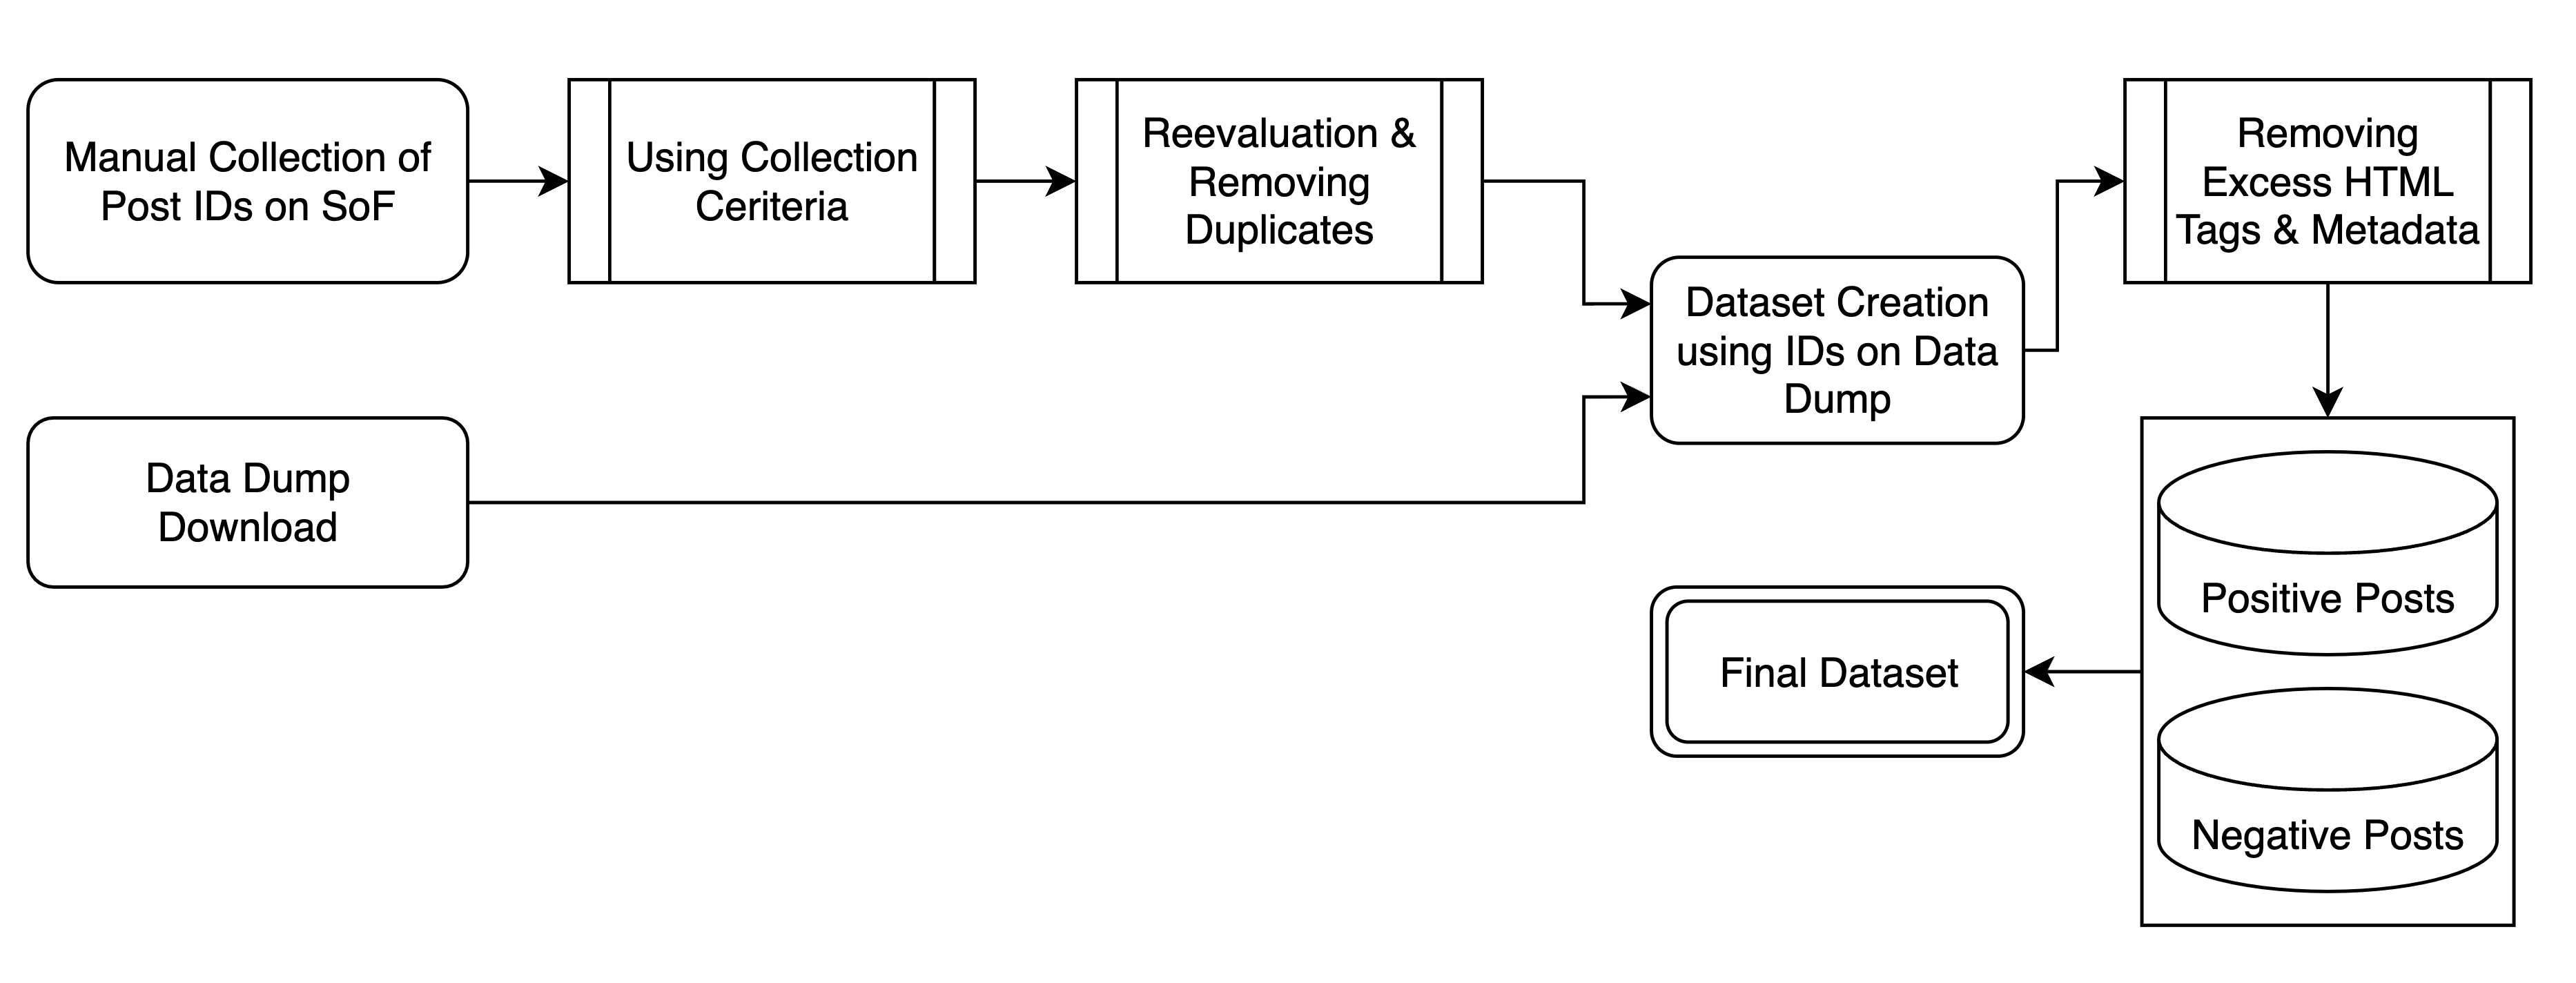
\includegraphics[width=1\textwidth]{images/figure1.png}
  \caption{Dataset Creation}
  \label{fig:figure41}
\end{figure}

\begin{figure}[h]
  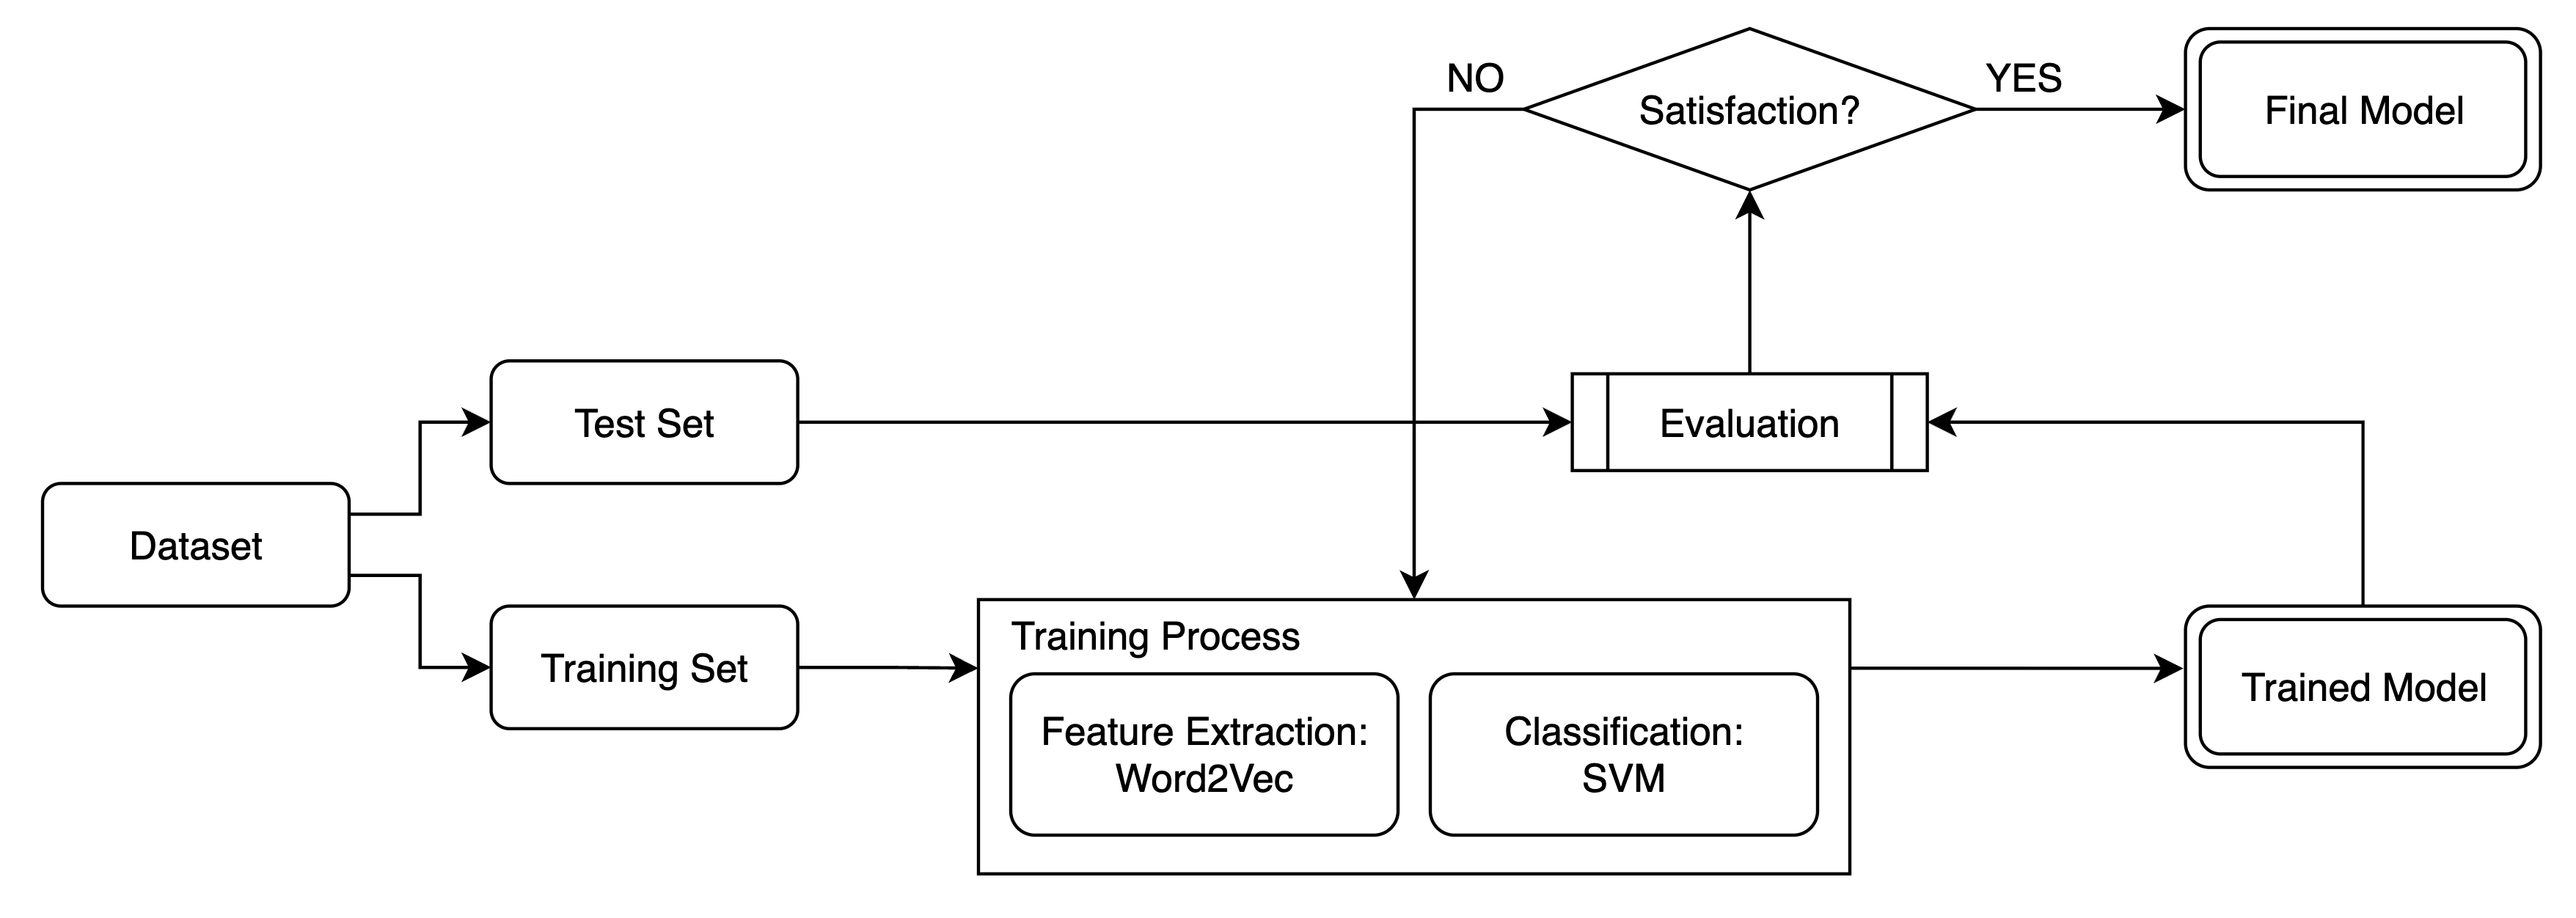
\includegraphics[width=1\textwidth]{images/figure2.png}
  \caption{Experiment 1: Creation of CM-PaCE model}
  \label{fig:figure42}
\end{figure}

\begin{figure}[h]
  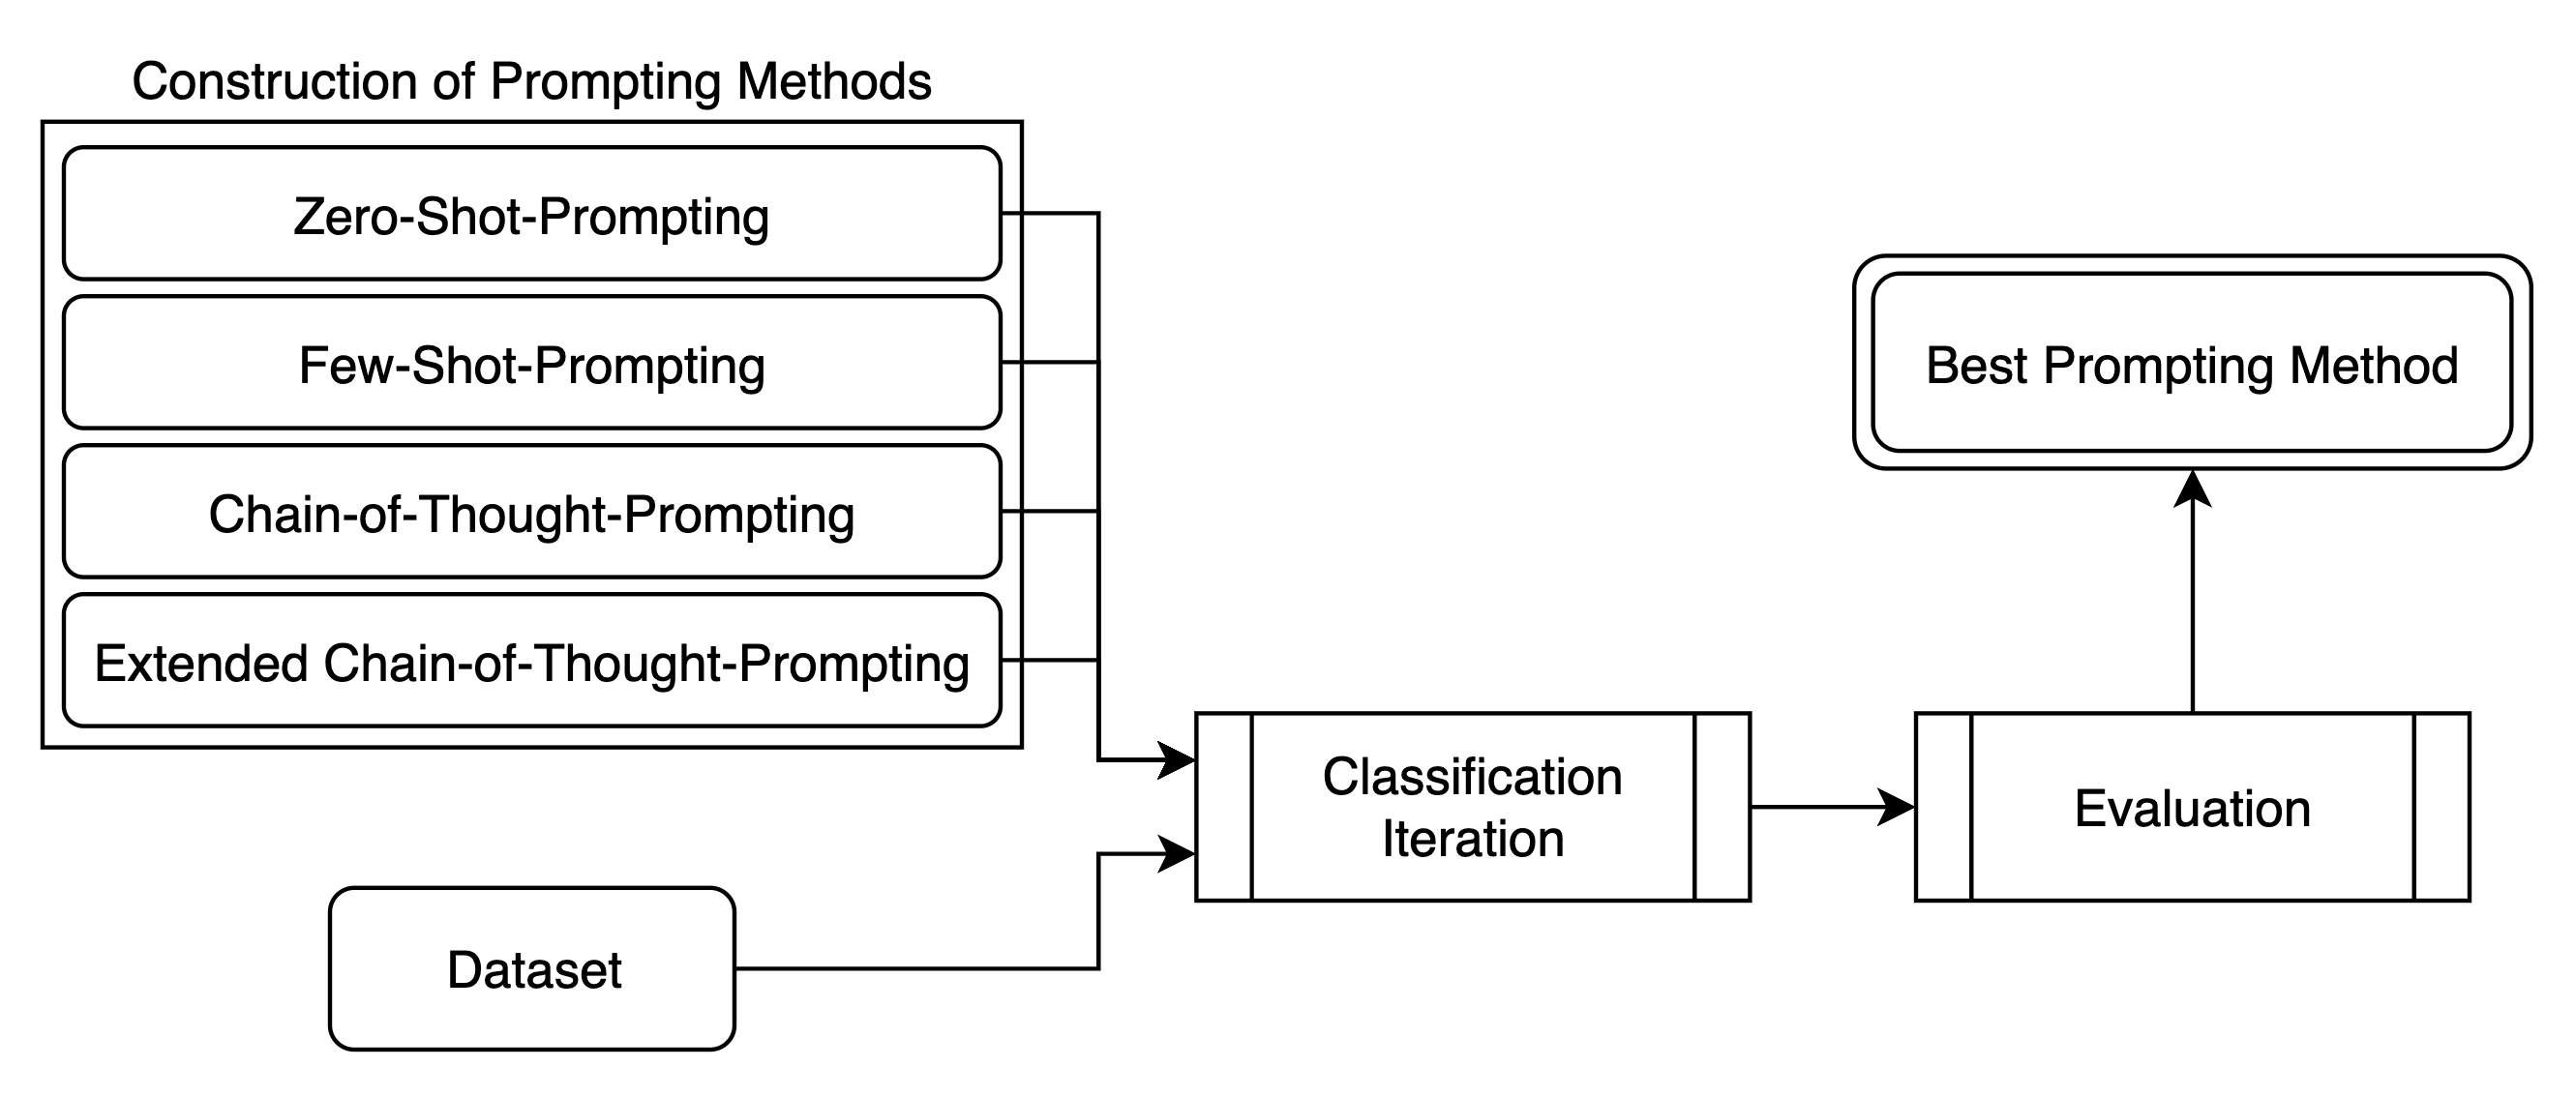
\includegraphics[width=1\textwidth]{images/figure3.png}
  \caption{Experiment 2: Using LLM for Classification Task}
  \label{fig:figure43}
\end{figure}

\begin{figure}[h]
  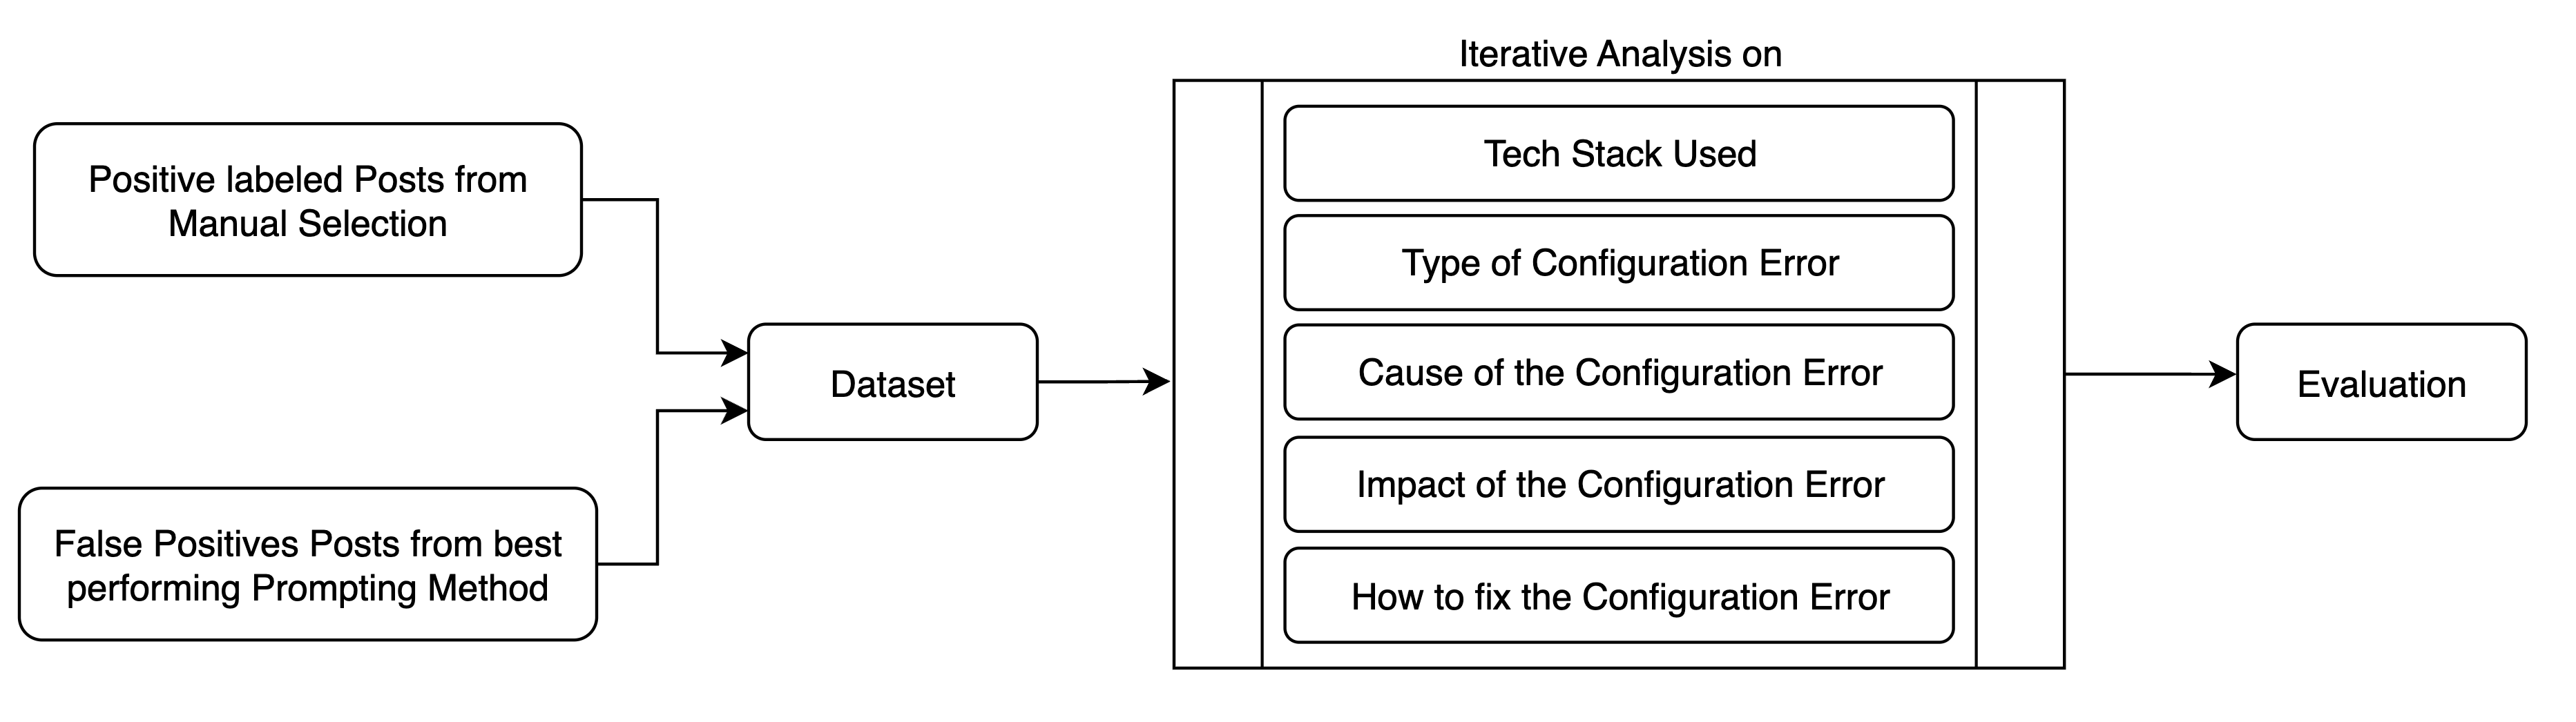
\includegraphics[width=1\textwidth]{images/figure4.png}
  \caption{Experiment 3: Analysis utilizing LLM}
  \label{fig:figure44}
\end{figure}

\section{Dataset Creation}
The goal is to collect Stack Overflow (SoF) posts that can be used to train the model to detect configuration errors 
in those posts. After successfully training the model, it should be given another set of posts to evaluate its effectiveness. Since we are using an unsupervised machine learning approach, we had to manually label each collected post as either True or False, indicating whether the post is indeed related to configuration errors according to our criteria.

\subsubsection{The Data Source}
To collect the posts for our dataset, we decided to take an official data dump of Stack Overflow, which can be found 
on archive.org (\citet{stackexchange:2023}), provided by Stack Exchange, Inc. Using this data dump, we crawled and parsed the collected posts into our own dataset. Each post had various metadata, such as an unique ID, a title, a creation date, and more. For our purposes, only the title, ID, score (user rating of the original post), and body were of interest. The rest of the metadata is still open for future research and optimization of the model, such as the number of views to further improve the retrieval of relevant posts. At the time of this work, the posts ranged from July 2008 to the most recent posts in the data dump, which are from March 2023. From these posts, we proceeded to extract our collection of posts for the training and test sets.

\subsubsection{Collection Criteria}
For the criteria to manually collect our dataset, we considered the work of \citet{tian:2020}. The authors had a similar 
task to ours, where they tested different machine learning methods to identify architecture smells in Stack Overflow posts. The authors collected 395 posts for their training and test set, also split 90/10. This assured us that our goal of 500 posts might be enough for the task. Next, the authors proposed seven criteria by which they decided whether a post was positively labeled (architecture smell related) or not. After testing some of these criteria with minor modifications to fit our domain, we decided to modify each criterion to consider configuration errors instead. This gave us a set of seven criteria to manually collect the posts for our dataset, presented in Figure \ref{fig:figure499}. Each post is labeled `True' if at least one criterion for related posts applies, while the post is labeled `False' if criterion C7 applies.

\begin{figure}[h]
  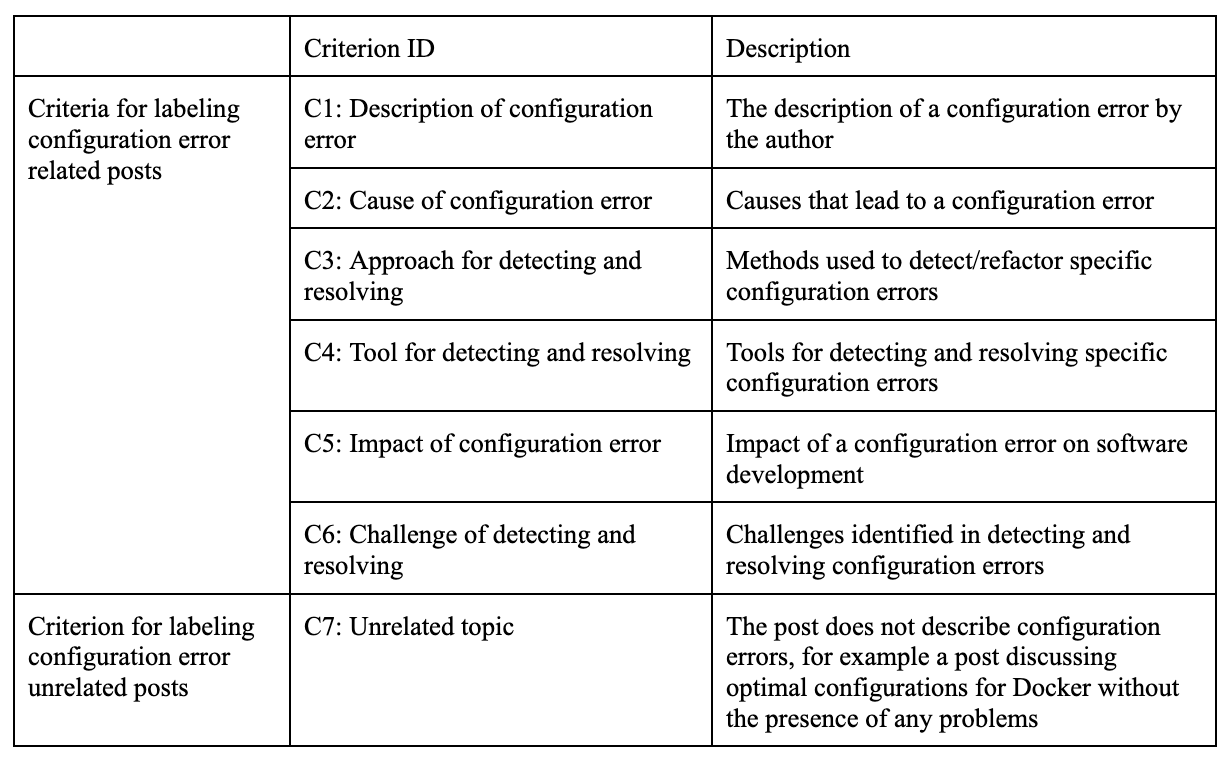
\includegraphics[width=1\textwidth]{images/criterions.png}
  \caption{Overview of the criterions used for the selection process}
  \label{fig:figure499}
\end{figure}

These criteria helped us decide which posts to include in our dataset. Building on them, they provide a reliable 
decision-making tool for the task of manually collecting the posts from Stack Overflow. While the negatively labeled posts have only one criterion, that the post does not contain a talk about configuration errors, it still contains a variety of similar posts, such as talks about configuration in general. In this way, we can exclude posts that contain the topic of configuration for conversations that are not related to specific errors. We made this decision to train the model not just on configuration keywords like `configuration', `config file', or services like `springboot', but to train the model on the specific features of a configuration error post. This reduces the risk of the model predicting the `true' label for posts that do not contain errors at all, such as discussions about the most efficient configuration tool for a given application. We also decided to include vague or difficult to understand posts to challenge the model's decisiveness in the process.

For the manual selection of posts, we decided to use the Stack Overflow website, taking advantage of the search engine 
to retrieve posts to apply the criteria to. This makes the process of finding posts for the training set easier than manually searching on the raw data dump. The data dump will then be used to work on the full posts with their metadata. We set some keywords to get a set of posts to apply the criteria to. For the positive posts that we labeled as containing configuration error discussions, we set the following keywords to search for on the site: configuration error, configuration, configuration file. After selecting a post from the search results, we used the ``Find and Replace'' tool in our browser to search for keywords such as config, which gave us a good view of the sentences indicating whether the post met our criteria. For each selected post that we included in our collection, we wrote down the specific post ID from the SoF website to later crawl the posts in the full dataset. Applying the criteria to the search results from Stack Overflow for these keywords, we collected an initial set of 270 posts for the label `True', which after further filtering was reduced to 261 posts.

For the negative posts that do not contain talk about configuration errors, we chose the following keywords: 
configuration, docker, golang, angular, sql, rust, aws, azure. We chose these keywords because they form a good basis for collecting posts that have something to do with configuration, but not configuration errors (Golang, as a cloud backend language, is a good keyword to find such posts), and posts that have nothing to do with configuration at all. We collected an initial set of 271 posts for the `False' label, which was later reduced to 241 posts. Thus, we collected a total of 541 posts, which shrank to 502 posts after eliminating duplicates and re-evaluating the posts.

We chose this number of posts to ensure our dataset contains a sufficient amount of heterogeneous data enabling proper model training. Although the dataset is sufficiently large, additional data points have the potential to enhance the model's performance on complex data. We set a target of collecting approximately 500 posts, which resulted in a dataset of 502 posts. While having more posts may improve the model, the time required to manually collect them limited our dataset to this size. To split the dataset into the desired 90\% training posts and 10\% test posts, we utilized the sklearn library in Python (\citeauthor{scikitlearn}).

\subsubsection{Preprocessing}
After collecting the ids of posts for our training set from Stack Overflow, we iterated on the data dump to create a 
full training set of these posts. Since the Stack Overflow data dump includes complete posts with metadata and HTML tags, preprocessing is necessary to prepare the data for model training. To achieve this aim, we formatted each entry from the manual selection to the desired format for our model. The final format includes only the body and our contributed label, which is True or False. We have saved all posts that matched the post IDs from the collection process. After completing this step, we obtained two datasets, each consisting of posts labeled as positive or negative, along with their respective metadata. We proceeded to format the body of these posts by removing any html tags as well as double quotation marks that interfere with the XML format. Finally, we merged both datasets to create the final dataset, which solely comprises the cleaned body and label. This final dataset will be utilized during the training process.

\section{Experiment 1: CM-PaCE Approach}
\subsubsection{Word2Vec}
We selected Word2Vec to extract features from Stack Overflow posts because it was more suitable for the task and 
considers the context of words. Word2Vec utilizes word embeddings, which are vector representations of words that effectively capture semantic and syntactic relationships. This is particularly beneficial for small documents with sparse information on unknown words. Word2Vec is a reliable and scalable algorithm, which is ideal for our purpose (\citet{mikolov:2013}). As previously discussed, we chose the Skip-Gram model due to its suitability for predicting the surrounding context words for a given word.

To implement the Word2Vec algorithm, we utilized the gensim library in Python (\citet{rehurek:2022}). This open-source library offers 
many models for natural language processing tasks, including topic modeling and information retrieval. While Word2Vec is a popular NLP algorithm, it is only one implementation, and gensim is an excellent tool for developing our feature extraction model. The Word2Vec model in the gensim library is customizable through its hyperparameters and can take a set of documents as input (\citet{rehurek:word2vec}). The resultant output comes in the form of word vectors which numerically represent the semantic and syntactic relationships between words. Put simply, after creating a lexicon of words from the corpus, these vectors signify the importance of words via numerical values. Gensim's vectors permit word comparison and yield a numerical value indicating the word pair's relationship. These vectors also rank the most similar words for a given target word based on their numerical proximity. They demonstrate each word's contextual significance and are key in training a sentence classification SVM model.

To further explain the mathematical workings of this model, envision it as a basic neural network consisting of an 
input layer, hidden layers, and an output layer.  The input and output vectors are identical in size, representing each word in the dictionary as a single representation in the input layer. The output layer encompasses all words in the dictionary. Once the model is trained, the output layer displays the relationship to the input words. For instance, if we have one word, such as `Candle', its corresponding position in the input layer will be 1, and all others will be 0. The trained model will then display the probability of relevance to this word, beginning with the first word alphabetically in the dictionary. This matrix of relationships arises from the training process, which trains the model on neighboring words using a window to generate context for each word.

We processed each post from the dataset file using a pre-processing function and a filter to achieve our desired 
output. The function tokenized each post, separating the text into individual words. All words were converted to lowercase, and we removed punctuation, numbers, and excess white space. Though html tags were removed, the filter also double-checked for tags to drop. We then removed stop words, using the standard stop word collection provided by gensim. The sentence words have been stemmed to capture context among words that share a topic. For instance, our algorithm stems the term ``configuration'' to ``configur'', enabling us to capture all related forms such as ``configuring'' or ``configured''. By doing so, we can effectively grasp the context of phrases like ``After configuring the file I got this error''. The resultant sentences are then placed in a set along with their corresponding labels. This way, we possess lists of words designated with True or False labels. The complete set is divided into a training set and a test set, utilizing the appropriate function from the sklearn library. We chose to divide the dataset with a 90/10 split, and using the sklearn function, it obviates the biases by shuffling the data and ensuring that each set has an equitable distribution of both labels. Though some bias may still exist due to the random data split used for better model training than other splits.

The Word2Vec model provided by gensim utilizes a range of hyperparameters. In the following, we will discuss the 
specific hyperparameters that were configured for our model and their significance. Additionally, we will provide information on the selection criteria used for the final hyperparameters and their corresponding values. To ensure separation, hyperparameters are predetermined prior to the training process, while plain parameters, including weights in the neural network, are adjusted by the model.

\begin{itemize}
  \item \textbf{min\_count:} This parameter establishes the minimum frequency required for a word to be considered in 
  the preprocessed corpus by the model.  Any words with a frequency below this threshold are discarded, which eliminates irrelevant noise generated from infrequent words. Raising this threshold value aids in noise reduction for words that occur once in the corpus.
  \item \textbf{alpha:} This parameter, also known as the learning rate, controls the size of the steps the model 
  takes as it moves toward a solution. A higher learning rate indicates that the model will take larger steps, which can lead to a better solution faster. Conversely, a greater learning rate also entails a greater tendency to overfit and produce poorer results on unseen information. On the other hand, a lower learning rate can help to train the model more accurately, which may cause the model to take longer to find the best solution.
  \item \textbf{sg:} This variable determines whether the model will use the Skip-Gram training algorithm. A value of one indicates the use of Skip-Gram, while any other value indicates the use of the Continuous Bag of Words (CBOW) method.
  \item \textbf{hs:} Setting this value to 1 enables the model to implement hierarchical softmax during the training process. Hierarchical softmax is a more efficient technique for training a Word2Vec model compared to the traditional softmax function. This approach represents the vocabulary as a binary tree with each leaf node being a word. The probability of a word is calculated by traversing the tree from the root node to the corresponding leaf node. Utilizing this method for smaller datasets like ours has the potential to enhance the model's accuracy.
  \item \textbf{window:} The window parameter determines the size of the sliding frame used by the model to traverse the word corpus. The frame is positioned over the sentence, capturing only the adjacent n words to learn the word vector. While larger window sizes enable the model to capture more contextual information around a target word, it may increase the risk of overfitting on smaller datasets.
  \item \textbf{epochs:} This parameter determines the number of iterations for the model training process. During each iteration, the model adjusts the word vectors by predicting the context words for the target word, and updating the word vectors of the target and context words based on these predictions. If the number of iterations is insufficient, the model will not have adequate time to adjust and attain a high level of accuracy. On the contrary, excessive iterations may result in overfitting as the model is trained solely on the precise words of the training dataset.
\end{itemize}

To evaluate the performance of our model's Word2Vec component, we conducted an analysis of the model's output within 
our domain. For this purpose, we utilized the word vector representation from the model to generate a list of the top 11 words with the highest relevance in the corpus. This enables visualization of the general topic of our dataset and evaluation of the initial results for accuracy. For instance, according to the Word2Vec model, good performance is indicated by the inclusion of top words like ``configuration'' (stemmed to ``configur''), ``error'', and other related terms associated with configuration errors. The training set is biased towards the topic of configuration, which encompasses posts that mention configuration without errors, resulting in ``configur'' being favored in the higher ranks. To determine the efficacy of the model, one can identify the most related words for a target word generated by the model. Gensim, as previously mentioned, provides access to various functions for processing word vectors and obtaining the most related words for a target. Through this method, it becomes feasible to assess the contextual validity of the model by correlating typical words in the domain of configuration errors to one another. For example, the term ``error'' was consistently the most related to ``configur'' across all hyperparameter variations, confirming the model's functionality.

After conducting manual tests with various combinations of hyperparameters in our initial models, we identified a set 
of hyperparameters which produced satisfactory results for different models trained on shuffled training sets in our domain. We maintained a record of each hyperparameter set by logging their values and the similarity results between terms like ``configur'' and ``error'', and then analyzing the most similar terms for the target words ``config'' and ``configur''. As a result, we settled on the following hyperparameters for the Word2Vec model in our top-performing models.\\

\begin{adjustwidth}{1cm}{0cm}
`min\_count': 5\\
`alpha': 0.01\\
`sg': 1\\
`hs': 1\\
`window': 4\\
`epochs': 500\\
\end{adjustwidth}

We achieved the best models through multiple trials based on our manual testing method. We selected a ``prime'' model 
using these values for our final Word2Vec model. This model processes input posts in the same manner as the training process, including tokenization, stemming, preprocessing, and transformation of each word into its respective word vector. The result of this section of the final model will be a group of word vectors representing the word embeddings of the entirely preprocessed post. By utilizing these word vectors, we can employ the classification model to obtain an output for every post.

\subsubsection{SVM}
For the classification task, a SVM model utilizes feature vectors, akin to those produced by the Word2Vec model. To 
evaluate the model's output, each document is presented with a label during the training process. For our corpus, we assigned ``True'' and ``False'' labels to each document, specifically to each post. The objective of the SVM model is to identify the hyperplane that maximizes the margin- the gap between the hyperplane that divides the two classes and the nearest data points from each class. A higher margin implies better generalization of the hyperplane to novel data, but a larger margin also increases the risk of overfitting the training data. For classification, the SVM converts input vectors into a high-dimensional feature space by using a kernel function. The algorithm locates a hyperplane to distinguish between the two document classes and allows for a sufficient margin to avoid overfitting. The labels attached to each document inform the model about its result during the last iteration, which helps adjust the weights of the neural network. Once the model is trained, we will examine its effectiveness by measuring accuracy, precision, recall, and F1 score through a test set. This method involves tallying the true negatives and true positives, which were correctly classified by the model from the test set. Similarly, we add the false negatives and false positives, which were erroneously classified by the model from the test set. To create and employ our own SVM model, we will utilize the SVM techniques available in the Python library \citet{scikit:svm}.

Our final model consists of two parts: the Word2Vec model and the SVM model. We linked these models by utilizing the 
output object of the Word2Vec model to transform each sentence into feature vectors. A crucial aspect to consider when connecting these models is the differing feature lengths. As sentences produce a higher-dimensional matrix of word embeddings, we must flatten the matrix in a manner that allows the SVM model to use it effectively. This is because the SVM model expects a single input vector. Thus, we parse the vectors into the SVM model for training purposes. After establishing the connection between both models and implementing the SVM model from the sklearn library, selecting the appropriate hyperparameters becomes necessary.

The SVM model requires various hyperparameters for its application. The following hyperparameters are specified and 
configured for our model.

\begin{itemize}
  \item \textbf{C:} This parameter regulates the model by controlling the trade-off between minimizing training error and maximizing margin. Put simply, a larger C value directs the model to prioritize minimizing training error, which can result in overfitting. Conversely, a smaller C value directs the model to prioritize maximizing margin, which may result in underfitting.
  \item \textbf{Gamma:} This parameter is solely applicable to non-linear kernels, as it regulates the impact of support vectors on the decision boundary. Increased gamma values amplify the support vectors' influence, potentially resulting in overfitting if set excessively high. Conversely, decreased gamma values reduce the support vectors' influence, potentially resulting in underfitting, where the model cannot discern enough context to classify the input accurately.
  \item \textbf{Kernel:} The kernel function transforms input vectors into a higher-dimensional space. Four types of 
  kernel functions exist: `linear', `poly', `rbf', and `sigmoid'. The linear kernel function returns the dot product of the two input vectors. The polynomial kernel function uses the polynomial of the two input vectors to a specified degree. The rbf kernel returns the exponential of the negative squared Euclidean distance between two input vectors and is significantly affected by the gamma value. Finally, the sigmoid kernel function utilizes the hyperbolic tangent of the dot product of the two input vectors.
\end{itemize}

To determine optimal hyperparameters, we utilized the GridSearchCV method provided by sklearn. This technique 
exhaustively traverses a predefined grid of hyperparameter values for every possible combination. The model is then trained and assessed on an independent validation set for each parameter combination. The optimal set of hyperparameters is selected based on the combination of parameters that yields the best-performing model. We opted not to specify the iteration for the model since it has an inbuilt method to ascertain convergence. Additionally, adding this fourth value would drastically increase the complexity of using grid search. Below is the parameter grid specified for our grid search method:\\

\begin{adjustwidth}{1cm}{0cm}
  `C': [0.001, 0.005, 0.01, 0.02, 0.05]\\
`gamma': [0.001, 0.01, 0.1, 1, 10]\\
`kernel': [`linear', `poly', `rbf', `sigmoid']\\
\end{adjustwidth}

Every combination of these parameters is evaluated by the sklearn approach based on its internal score and loss. After 
running this grid search on the specified values, the model resulted in the best score with these hyperparameters settings: [C: 0.005, gamma: 0.001, kernel: `linear']. After testing more iterations, we changed the `C' value to 0.01 because it yielded better results for the tech-specific complexity. Even though the gamma value is not mandatory for the linear kernel function, we retained it for consistency purposes. As with the Word2Vec part of our model, we also logged the training process for the SVM model. This way, we can compare past attempts, determine performance differences, and assess the most effective model based on results.

After completing the training process, the performance of each model is assessed by evaluating its accuracy, 
precision, recall, and F1 score using a separate test set created earlier. This evaluation is carried out on unseen data to determine whether each label is classified successfully. The evaluation results are then used to identify areas where the model can be improved. By evaluating the model on a reserved test set, we can obtain an impartial evaluation of its performance on unobserved data. This information can enhance the model and facilitate informed decisions about its implementation in practical scenarios. Additionally, it is critical to test the model for overfitting, wherein the training process shows promise, but the model underperforms on unobserved data.

\subsubsection{The CM-PaCE Model}
To complete our final machine learning model, we combined both the Word2Vec part and the SVM part. The Word2Vec model 
output was utilized to generate input for the SVM model, which involved converting input sentences into feature vectors. This approach turns the Word2Vec model into a preprocessor that transforms the input into vectors representing each post's context with respect to configuration errors. The SVM model identifies features that provide context for configuration errors. It is utilized in the trained model to classify input posts as either `True' or `False'.

The CM-PaCE (Classification Model for Posts about Configuration Errors) model is currently used to categorize posts 
pertaining to configuration errors. The Word2Vec component converts each input into feature vectors, which are subsequently analyzed by the SVM component to identify any discussion of configuration errors. Following some sample trials, we confirmed that the script is fully compliant with our anticipated performance, successfully accepting input and providing output.

\section{Experiment 2: LLM Approach}
Recent advances in large language models (LLMs) have led to a significant growth of opportunities for applying machine 
learning in various fields. LLMs, such as ChatGPT, are well-suited for advanced fields such as configuration errors, as they allow for training on domain-specific data. Pre-trained models with a greater knowledge base than standard NLP models are accessible to all via API use. The classification process can be challenging, particularly for small models like our CM-PaCE model. In this second approach, we demonstrate how LLMs, specifically the gpt3.5-turbo model (\citeauthor{openai:2023}), can be employed to classify posts containing discussions about configuration errors, similar to our classification model. Furthermore, we will utilize NLP's functionality to provide input feedback, which will aid in comprehending how the model arrived at its conclusion. To achieve optimal results, we will evaluate various prompt engineering techniques to find the most effective prompt for our study's model.

Further data preprocessing is unnecessary for this approach. The dataset we previously created is adequate to iterate 
on this model and there is no requirement to preprocess each document entry by removing stop words or tokenizing the text. Following the creation of the dataset, we removed most of the HTML tags. However, we retained some tags like href links and code tags to provide the model with contextual information regarding the structure of the post. The dataset will be further separated to test different prompting methods, where the Few-Shot prompting method will need some examples from the dataset for the initial prompt. This method will have four posts --- two positive and two negative --- as examples, which will be removed from the dataset for consistency with the other methods. That way, all Prompting methods contain the same training data, while the Few-Shot prompting method will get four examples to start with. The remaining 497 posts will be used to evaluate the model in all prompting methods.

During the iteration process, we will input the text of each document into the prompting function, which will 
subsequently assess the API and produce an output from the model. This output is manually reviewed and recorded in a table alongside the original label for each document. This enables us to generate measurement scores by assessing the output label generated by the LLM model against the actual label assigned to each document. Since a high accuracy of the model is assumed, we include the number of tokens used for each method as a secondary measurement, specifically for getting the efficiency.

The gpt3.5-turbo model works by creating http requests to the API with several parameters. For our approach, we 
decided to specify only the temperature parameter because it directly affects the randomness of the model (\citeauthor{openaicomplete:2023}), which we want to reduce to get the best results. Typically, a higher temperature (up to a value of 2) is utilized to produce diverse outputs, such as generating more natural responses to common questions or exhibiting some degree of ``creativity'' in producing texts such as poems. Lower temperatures (as low as a value of 0) can result in more stable and predictable outcomes, aligning with our objective of accurately classifying posts and emphasizing the provided information. Additionally, this can decrease the likelihood of model hallucinations, in which it generates random outputs that do not align with the input.

\subsubsection{API Call \& Functions}
For each iteration in the evaluation process, we utilize OpenAI's API for gpt3.5-turbo. The API is directly accessible 
through Leipzig University, utilizing the gpt3.5-turbo model. Each prompt involves sending a post request to the server, with a specified API key header and a JSON object containing the content for the call. The JSON object includes an array of messages and parameters. In our case, we have two types of messages: the system role message, which defines the actions the model should take, and the user role message, which allows the user to input information to be processed. These are separate prompts for the model, with the system prompt always being ``Pre-training'', which we aim to construct and not change in the final model. The user prompt, on the other hand, serves as the varying input for the iterations.

In the version used in this experiment (gpt-3.5-turbo-0613), the API call response is a JSON object that includes a 
`choices' object, the date of creation, the call's id, the model used, the method of model use, and a usage object featuring the number of tokens utilized. Of particular interest for our intention is the `choices' object, which incorporates the messages array that the model produced, in addition to the finish reason and index where the model ceased function. In this case, the messages array comprises a single message with the role attribute labeled as `assistant' and the message content serves as the actual output we need to evaluate.

We utilized the `requests' library by \citeauthor{reitz:nd} within our Python code to generate post requests to the API. 
Each post request undergoes parsing with the constructed prompt as the system role message and the user input as the user role message in the messages array. The API key and the URL for the post request are saved in a distinct file. We developed a simple function that can be called with the designed prompt and the input to return a response for the output. Additional functions for our implementation consist of logging results, along with the token size and input, in a log file, and selecting specific documents from the dataset for distinct stages of the experiment.

\subsubsection{Prompt Engineering}
In the \ref{sec:pe} section, we introduced the three prompting methods we will employ in our study: 
Zero-Shot prompting, Few-Shot prompting, and Chain-of-Thought prompting. After evaluating each method using our dataset, we determined which one is best suited for retrieving posts about configuration errors. The following are the prompts for each method, which we will use to iterate on the documents. Note that our constructed prompt is provided as the role of each API call, telling the model what task it has to accomplish.

\begin{itemize}
  \item \textbf{Zero-Shot prompting:} In this prompt (see Appendix \ref{fig:figure45}), we have provided information on the domain and format of posts that the model will encounter as input to recognize keywords that indicate code fragments. However, we did not offer any concrete examples of positive or negative inputs, resulting in the model having no pre-training in the form of ``shots'' and relying solely on Zero-Shot prompting. Following the classification, the model must provide a brief explanation for its decision. It is important to note that this is a basic prompt intended to test the effectiveness of methods on small subsets before creating a more refined and comprehensive version.
  \item \textbf{Few-Shot prompting:} In this prompt (see Appendix \ref{fig:figure46}), four sample documents are provided, two with positive labels and two with negative labels. We omitted a specific subject matter to serve as a direct guide for the model on how a post should appear. By giving examples, Few-Shot prompting pre-trains the model to understand the expected output for a given input. Despite this, we still require the model to justify its decision. In the evaluation process, we had to exclude two documents from the dataset because the provided examples made the prompt too long for the model to work. Due to length limitations, we did not include the full post examples in the appendix. Refer to our Jupyter Notebook for the complete examples.
  \item \textbf{Chain-of-Thought prompting:} This prompt (see Appendix \ref{fig:figure47}) is similar to the first, where Zero-Shot prompting was used.  However, an additional instruction was included this time, leading the model to think in a step-by-step manner. As a result, the model devised a plan that incorporated more domain-specific knowledge to approach the result, potentially enhancing the understanding of posts prior to arriving at a decision. In brief, the model conducts a comprehensive analysis of the issue by referring to its experience with comparable problems, dissecting the problem into manageable parts, and producing a consistent and final resolution. We also used a second version of Chain-of-Thought prompting (see Appendix \ref{fig:figure48}), applying the criteria for positive documents from our manual selection process. This extended Chain-of-Thought prompting method served as the fourth approach in the second experiment.
\end{itemize}



\subsubsection{Result Measuring}
To assess the overall effectiveness of the various prompting methods, we used accuracy, precision, recall, and the F1 score. After logging each output of the model along with the original label of the document to the console, we manually noted the false negatives and false positives to calculate the measurement scores. We used a Python function to calculate measurements, inputting the size of the dataset in positive and negative documents and the quantity of false negatives and false positives. Additionally, we wanted to measure the number of tokens per method, but this only produced reliable results on smaller dataset samples due to technical issues such as the API not responding. As a result, the evaluation runtime encountered various crashes, losing the count of the used tokens.

\section{Experiment 3: Dataset Analysis}

To emphasize the significance of accurately retrieving Stack Overflow posts related to configuration 
errors, we conducted a third experiment. We used the LLM model gpt3.5-turbo to analyze the retrieved posts from the Few-Shot prompting method, testing the model's effectiveness in not only collecting posts on a given topic but also examining the document for specific information. For each post, we asked the model to extract five aspects: the tech stack used, the type of configuration error, the cause of the configuration error, and how to resolve the configuration error. After collecting the responses, we manually verified them using our experience and knowledge of the field or with the help of verified answers on Stack Overflow to validate their accuracy.

The dataset for this experiment comprises the posts that we manually labeled as true, including those 
classified by the model as true positives and the few false negatives where the model incorrectly labeled true posts as not containing talk about configuration errors. To test the model's liability, we included the false positives from the previous experiment, in which the LLM mislabeled posts as containing configuration errors when we concluded that they did not. This could also reveal instances of human error, where we mistakenly labeled posts as not containing configuration errors. Overall, this reinforces the model's effectiveness in the retrieval process.

After manually evaluating the results in a qualitative study, we will measure the performance of the 
model by assigning points to correctly analyzed aspects. Each post can receive a maximum score of five points if all five aspects are correctly analyzed, and a minimum score of zero points if the model does not provide any valuable information on any of the five aspects. We decided to not give a point to an aspect if the answer of the model is either wrong or does not contain any information, as in stating that no answer can be found. After scoring each post, we will compare the performance on manually retrieved positive posts, false positives labeled by the model, and the overall dataset containing both positive posts and false positives.

\subsubsection{Aspects of Analysis}

This section discusses the selected aspects for analysis by the model. For each aspect, we will describe 
its importance for the task, provide a brief description of the aspect and its usefulness, and evaluate its overall usefulness for research or users.

\begin{itemize}
  \item \textbf{Tech Stack Used:} This aspect deals with information about the technology that can be found in the Post. This includes programming languages, frameworks, databases, containerization, operating systems, version control tools, development environments, and network technologies mentioned by the author. This aspect is useful to better categorize the configuration error or to separate similar configuration errors in detail, such as different versions of a framework where the error occurs in one version but not in an earlier version. It is also useful when identifying a solution for the error that can be found through simple strategies, such as using a different version of a programming language due to deprecated tools.
  \item \textbf{Type of Configuration Error:} What information can be found in the post on the type of configuration error. Is it a missing configuration parameter, an invalid configuration value, or a conflict between two configuration settings? Earlier, we discussed the three categories of configuration errors: parameter misconfigurations, software incompatibility, and component misconfiguration. This aspect is useful for categorizing the error and understanding how it occurred. By eliminating certain causes for certain types of configuration errors, the process of resolving the error becomes more manageable. For instance, if the issue is a parameter misconfiguration, the troubleshooting process should focus on that particular aspect of the configuration.
  \item \textbf{Cause of the Configuration Error:} What caused the configuration error? As with all aspects, this information can only be guessed in some cases, but if the post does not provide any information, we will rate the answer with no point. The cause of the error may range from typos to a misunderstanding of the configuration documentation or a bug in the software. This aspect is crucial because the author may provide an error message or other information that directly points to the cause of the error, making it much easier to resolve the issue. When encountering a similar configuration error as in the post, the user can also attempt similar solutions resulting from this cause.
  \item \textbf{Impact of the Configuration Error:} This aspect can be answered more thoroughly by addressing the author's stated problem and providing suggestions for similar cases, such as downtime or system crashes. It is particularly useful for researching and investigating configuration errors. To better prepare for potential scenarios, it is helpful to gain an understanding of the potential issues that may arise from a known group of configuration errors. For instance, when utilizing a particular version of a containerization tool, users should be aware of the potential impact that errors within the tool can have.
  \item \textbf{How to fix the Configuration Error:} This aspect is noteworthy because the model does not require any information from the post, as most posts do not provide an answer. Therefore, the model is responsible for generating a potential solution for the error. This aspect can be difficult to evaluate, either due to our limited knowledge on the topic or the absence of the error on our machine to test the solution. Alternatively, it can be easy to evaluate if the post on Stack Overflow has an accepted answer that the original author deems helpful in resolving the issue. This aspect is particularly useful for users who encounter a similar problem to that of the post's author. Given the information available to an LLM, it is especially useful to receive a set of potential solutions to the problem, even if it only helps to narrow down the root cause.
\end{itemize}

\chapter{Results}\label{results}

This section presents the results of the study. First, we provide the results for the CM-PaCE model and its underlying Word2Vec and SVM models. Next, we present the measurement scores for the different prompting methods on the classification task for the second experiment. Finally, we present the results for the third experiment, where the LLM analyzed the dataset.\\

\section{Experiment 1: CM-PaCE Approach}

\subsubsection{Word2Vec}

In this section, we present the outcomes of our classification model, CM-PaCE, with a focus on its Word2Vec component. This component generates word vectors from our dataset, aiding in the comprehension of contextual relationships and emphasizing significant words. For instance, the vector for `configuration' (stemmed as `configur' in our model) is elaborated in Appendix 
\ref{fig:figure51}. The similarity between `configur' and `error' was measured using model.wv.similarity(`configur',`error') and resulted in a high score of 0.76458657, indicating a strong contextual relationship. 

Despite limited commonality in the domain of configuration errors, `configur' and `python' still showed a contextual similarity with a score of 0.03798087. This demonstrates the model's capability to accurately discern context. The similarity scores are based on cosine similarity, ranging from -1 to 1. A score of 1 represents high similarity, 0 represents no similarity, and -1 represents dissimilarity. For example, the words `configur' and `color' have a slightly opposing meaning with a low negative score of -0.020100988. This demonstrates the model's nuanced understanding of word relationships in the higher-dimensional field.

The model was trained using the following initial values during the training process:\\

\begin{adjustwidth}{1cm}{0cm}
  min\_count = 1\\
  alpha = 1\\
  min\_alpha = 0.1\\
  epochs = 100\\
\end{adjustwidth}

To evaluate the model's performance, we analyzed the contextual relevance of words related to 
`configur', a stemmed version of `configuration', which is crucial in understanding configuration errors. The analysis of the top 21 words related to `configur' yielded valuable insights into the model's semantic comprehension as can be seen in figure \ref{fig:figure52}.

\begin{figure}[h]
  \centering
  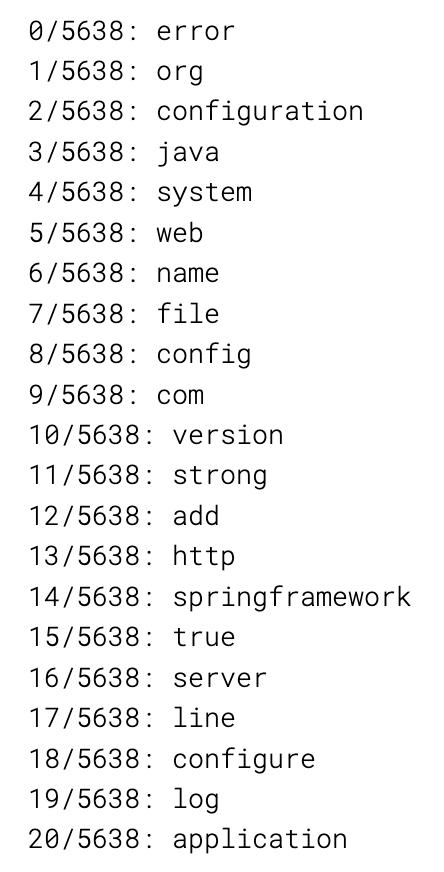
\includegraphics[width=0.4\textwidth]{images/ressimilar.png}
  \caption{Top 21 words related to `configur'}
  \label{fig:figure52}
\end{figure}

The results highlight that `error' is the most contextually similar word to `configur', in line with domain expectations, suggesting that the model effectively captures the link between configurations and errors. Other relevant terms such as `java', `system', `web', and `file' also emerged, which are typical in configuration error contexts. However, the high similarity with `org' requires careful interpretation due to its frequent but less direct relevance to `configur'.

During model refinement, we focused on improving semantic relevance rather than relying solely on syntactical co-occurrence. We adjusted parameters such as min\_alpha and revised our evaluation methodology. The initial training loss was 30488.695, which informed our adaptations for further iterations. The alpha value had a significant impact on this loss.

The Word2Vec model's parameters were iteratively modified, with a focus on the top 5 contextually similar words for `configur' and `error'. Built-in methods were used to assess common phrases in configuration error discussions. The adjustments included changing the number of training epochs, window size, and min\_count. The model's robustness was observed, particularly to min\_count variations. Significant changes were observed between 50 to 100 iterations, and after careful consideration, we selected 500 iterations at an alpha value of 0.01, as detailed in Appendix \ref{fig:figure54}. It was found that the model underfits at 50 iterations and overfits at 100, which negatively impacts similarity scores and item retrieval.

We did not observe any significant effect when altering the min\_count, so we chose a value of 5 to balance the word spectrum and minimize noise. Similarly, changing the window size had a negligible impact on the similarity scores between `config' and `error', and `configur' and `error', as shown in Figure \ref{fig:figure55}.

\begin{figure}[h]
  \centering
  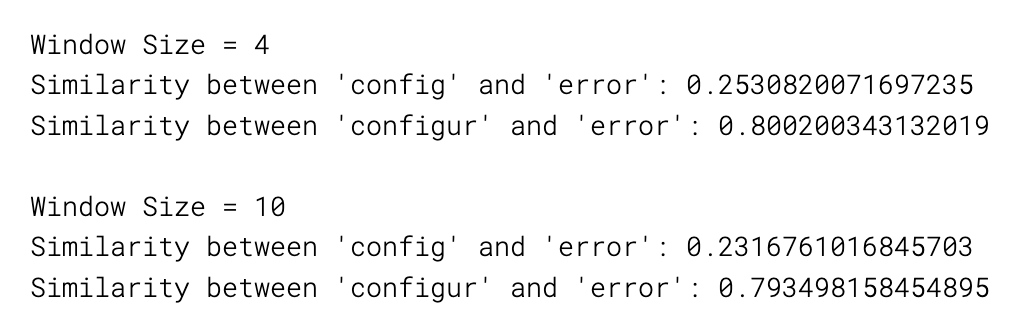
\includegraphics[width=0.9\textwidth]{images/windowres.png}
  \caption{Different Window Sizes impacting the similarity scores}
  \label{fig:figure55}
\end{figure}

The results suggest that the model has a consistent understanding of the relationship between `configur' 
and `error' regardless of the window size, as shown by the relatively high similarity scores. However, the scores between `config' and `error' were considerably lower, indicating that the model has a more nuanced and context-specific interpretation when different forms of the root word `config' are considered.

It is also noteworthy to highlight the interplay between the learning rate (alpha) and the other parameters by displaying the best result values of the similarity between `config' and `error' for various combinations of parameter values. See table \ref{tab:table51} for a comparison of different set alpha values on the `hierarchical softmax' and `Skip-Gram' values, as well as three different alpha values, impacting the similarity score between `config' and `error'.

\begin{table}[ht]
  \caption{Overview of different alpha, hs, and sg values impacting the similarity between `config' and `error'}
  \centering
  \begin{tabular}{c|cccc}\toprule
  Alpha & hs=0, sg=0 & hs=1, sg=0 & hs=0, sg=1 & hs=1, sg=1 \\ \cmidrule(l){1-5}
  0.01   & -       & -       & -       & 0.2317 \\
  0.001  & 0.4743  & 0.7955  & 0.8376  & 0.3497 \\
  0.0001 & -       & -       & -       & 0.3833 \\ \bottomrule
  \end{tabular}
  \label{tab:table51}
\end{table}

After rigorously iterating and optimizing the model parameters, specifically the alpha values in 
relation to other model settings, we identified the optimal configuration for our Word2Vec model. This fine-tuned model was then used as the primary input for the subsequent stage of our classification pipeline, the SVM method. The parameters of our Word2Vec model, as presented in the methodology, yielded the results in our evaluation process that are presented in Appendix \ref{fig:figure56}.

These findings are noteworthy. The moderate similarity score between `config' and `error' suggests a 
nuanced understanding of their relationship, while the high similarity score between `configur' and `error' highlights a more direct association in the context of configuration errors. The model's ability to discern relevant contextual associations is demonstrated by the array of most similar words for both `config' and `configur', which includes terms like `file', `error', and `occur' reflecting common elements in configuration error discussions. In a diagnostic exercise, the model accurately identified `java' as the outlier when presented with the set ['configur', `error', `invalid', `java', `problem', `cloud']. This result confirms the model's ability for semantic discrimination, which is crucial for nuanced language tasks such as classification.

Upon processing, the words `configur', `error', and `occur' were extracted, tokenized, and preprocessed 
from the sentence. These word vectors were then computed, providing a granular view of their semantic features and reflecting their complex semantic attributes within the context of the sentence. The feature vectors for the three tokens of the sentence in order can be seen in Appendix \ref{fig:appendix1}, together with the aggregated feature vector for the whole sentence in Appendix \ref{fig:appendix2}. This vector representation for sentences was then used to train the SVM model.

\subsubsection{SVM}

The primary objective of the SVM component in our CM-PaCE classification model was to use the generated feature vectors for classification after training on a designated dataset. To achieve this, we needed to identify the optimal set of hyperparameters, with particular emphasis on the `C' parameter in the context of the scikit-learn Python library. This parameter is a crucial factor in regularizing the model, balancing classification accuracy with model simplicity. A lower `C' value can improve margin and generalization capabilities, while a higher `C' value can minimize misclassifications, but may increase the risk of overfitting. Therefore, determining the optimal `C' value is essential for ensuring robust model performance. The impact of changing `C' using the `linear' kernel can be seen in Table \ref{tab:table50}.\\

\begin{table}[ht]
  \caption{Different C values using the `linear' kernel impacting the results}
  \centering
  \begin{tabular}{ccccc}\toprule
  C & Accuracy & Precision & Recall & F1 Score \\ \cmidrule(l){2-5}
  0.01    & 0.922       & 0.925       & 0.925 & 0.925 \\
  0.001  & 0.922  & 1.0  & 0.852 & 0.92 \\
  0.0001  & 0.824       & 0.95       & 0.703 & 0.809 \\
  0.00001    & 0.529       & 0.529       & 1.0 & 0.692 \\\bottomrule
  \end{tabular}
  \label{tab:table50}
\end{table}

The data indicate that a `C' value of 0.01 achieves an optimal balance, with an accuracy of 92.16\%, 
precision and recall both at 92.5\%, and an F1 score of 92.59\%. In contrast, a lower `C' value of 0.001, while achieving a precision of 100\%, results in a decline in recall to 85.19\%, indicating a trade-off between false positives and false negatives. Further reducing the `C' value to 0.0001 and 0.00001 results in a significant deterioration of model accuracy and precision. The lowest `C' value leads to a high recall of 100\%, but at the cost of significantly reduced accuracy and precision (52.94\% for both). These results emphasize the critical influence of the `C' parameter in the SVM training process and highlight its role in dictating the trade-offs between various performance metrics. After considering these results, we chose a value of 0.01 for `C' to maintain good results while also achieving more consistent classification.

After initially testing different `C' values, we decided to find the best hyperparameter configuration for our SVM model by using a comprehensive grid 
search, using the scikit-learn library. This systematic approach involved exploring a predefined range of hyperparameters exhaustively.\\\\

\begin{adjustwidth}{1cm}{0cm}
  `C': [0.001, 0.005, 0.01, 0.02, 0.05],\\
  `gamma': [0.001, 0.01, 0.1, 1, 10],\\
  `kernel': [`linear', `poly', `rbf', `sigmoid']\\
\end{adjustwidth}

The outcome of this grid search yielded a set of hyperparameters that were deemed most effective for our 
model: C=0.005, gamma=0.001, kernel='linear'. This particular combination suggests that a relatively lower complexity of the model (as indicated by a smaller `C' value) yielded the most effective performance. The values for gamma do not affect the results for the linear kernel. Upon further examination, it was discovered that a `C' value of 0.01, while not best value resulting from the grid search method, offered a better balance between model complexity and generalization capability. The model's enhanced performance metrics were observed to be more favorable at C=0.01 compared to other tested values, substantiating this finding. Therefore, 0.01 was adopted as the preferred value for the `C' parameter instead of the grid search result.

After evaluating various hyperparameters and using a shuffled training and test dataset, we identified 
the optimal hyperparameters for the SVM component in the CM-PaCE model as C: 0.01 and gamma: 0.001 with a linear kernel. The gamma parameter, although irrelevant in the linear kernel context, was included as an artifact from the training process that primarily pertains to other kernel types. This selection process aimed to balance the model's generalization ability against overfitting, a critical consideration in machine learning model optimization.

The performance of the SVM model, as integrated into our CM-PaCE framework, was assessed using the  metrics accuracy, precision, recall, and the F1 score.\\

\begin{adjustwidth}{1cm}{0cm}
  Accuracy: 0.9019607843137255\\
  Precision: 0.9090909090909091\\
  Recall: 0.8695652173913043\\
  F1 score: 0.888888888888889\\
\end{adjustwidth}

The model achieved a high level of proficiency, with an accuracy of approximately 90.2\%, indicating the 
proportion of correct predictions out of the total. Precision, the measure of relevance in the model's positive classifications, was recorded at about 90.9\%, indicating a high rate of true positives in the predictions. The model's recall, which measures its ability to identify all relevant instances, was approximately 87.0\%, indicating its effectiveness in capturing positive instances. Additionally, the F1 score, a harmonic mean of precision and recall, was approximately 88.9\%, demonstrating a balanced trade-off between precision and recall in the model. These performance metrics demonstrate the robustness and reliability of the SVM component in our CM-PaCE model, highlighting its effectiveness in accurately and consistently classifying data.

\subsubsection{CM-PaCE}

To demonstrate the effectiveness of our finalized CM-PaCE model, we analyze a sample document that represents a positively labeled Stack Overflow post about configuration errors. The post in question can be seen in Figure \ref{fig:figure59}

\begin{figure}[h]
  \centering
  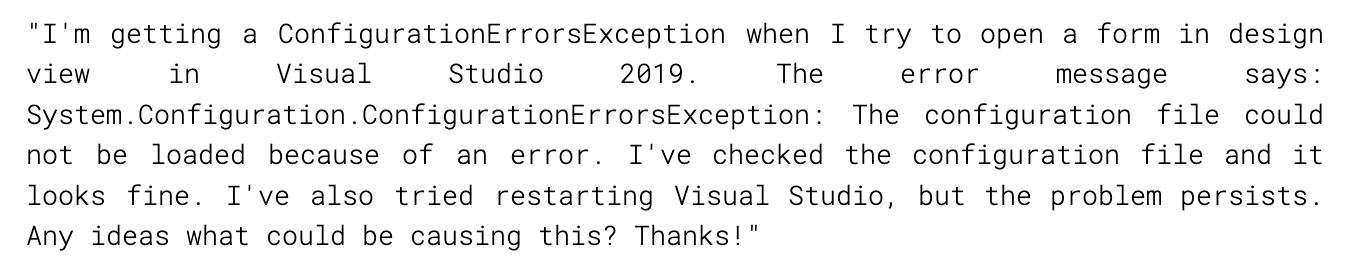
\includegraphics[width=1\textwidth]{images/examplepost.png}
  \caption{Example post to demonstrate the CM-PaCE model}
  \label{fig:figure59}
\end{figure}

When we use both the Word2Vec and SVM models combined to pipeline this document, the model returns 
`True', indicating that this is indeed a post about configuration errors. Furthermore, in order to rigorously test the capabilities of the model, we processed a series of additional documents, both manually sourced and self-authored, to simulate a diverse array of real-world scenarios and challenges that the model might encounter. The results confirmed the model's operational efficacy, as it consistently identified relevant posts with a high degree of accuracy. However, it is important to recognize the cases of misclassification, as shown in our previously discussed measurement results. Although these incidents were rare, they emphasize the need for ongoing refinement and adaptation of the model to improve its accuracy and dependability in different contexts. The iterative process of testing and refinement is essential to the evolution of our CM-PaCE model. It ensures its applicability and effectiveness in accurately categorizing Stack Overflow posts related to configuration errors.

\section{Experiment 2: LLM Approach}

In the second experiment, we utilized the LLM gpt3.5-turbo developed by OpenAI 
to examine the efficacy of various Prompt Engineering strategies in the context of classification tasks. Our approach involved deploying simple yet potent prompts to ascertain their effectiveness. The experiment's structure comprised an engineered prompt, serving as the `role', followed by an input. Consider the Zero-Shot prompting API call in Figure \ref{fig:figure511}, which consists of the role (the engineered prompt) and the input.

\begin{figure}[h]
  \centering
  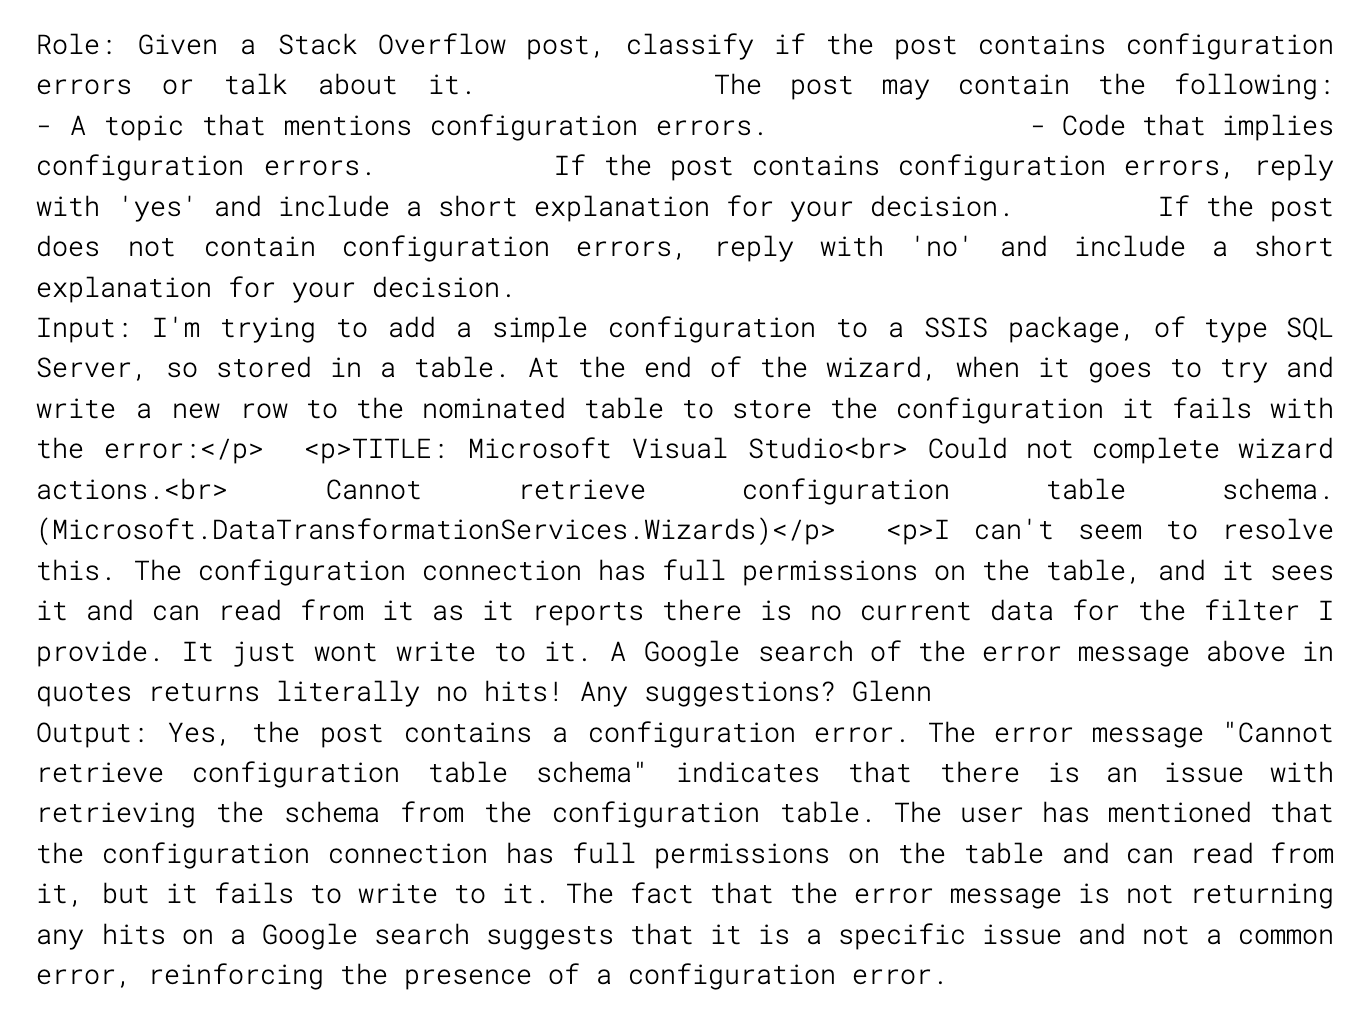
\includegraphics[width=1\textwidth]{images/llmextwo.png}
  \caption{Example for LLM reasoning on output}
  \label{fig:figure511}
\end{figure}

In the methodology section, we detailed the process of iterating over the complete dataset using the 
three distinct prompting methods, including the Chain-of-Thought method. We also included another version of the Chain-of-Thought method that integrates the criteria from our manual selection process. This integration aims to combine the systematic rigor of Chain-of-Thought with the nuanced insights from manual analysis. Table \ref{tab:table52} presents the results from this extensive iteration, which includes all three methods and their results in the four different measurement scores including the number of False Negatvies (FN) and False Positives (FP).

\begin{table}[ht]
  \caption{Overview of different measurement scores on the four prompting methods}
  \centering
  \begin{tabular}{cccccc}\toprule
   & FN / FP & Accuracy & Precision & Recall & F1 Score \\ \cmidrule(l){2-6}
  ZSP   & 0 / 62       & 0.875       & 0.807       & 1.0 & 0.893 \\
  FSP  & 1 / 36  & 0.925  & 0.877  & 0.996 & 0.933 \\
  CoTP & 0 / 56       & 0.887       & 0.822       & 1.0 & 0.902 \\
  Extended CoTP & 3 / 39       & 0.915       & 0.868       & 0.988 & 0.924 \\\bottomrule
  \end{tabular}
  \label{tab:table52}
\end{table}

The analysis of the results shows several key insights. Firstly, the Zero-Shot prompting method 
demonstrated perfect recall but exhibited a relatively high number of false positives, resulting in a precision of 80.69\%. This suggests that while the method is effective in identifying relevant documents, it also tends to overclassify documents as containing configuration errors. In contrast, the Few-Shot prompting method improved both precision and accuracy, indicating a more balanced classification capability. However, it is important to note that there was a slight reduction in recall and two documents were missing data due to API constraints, which are limitations of this approach.

The standard Chain-of-Thought prompting method showed identical recall to the Zero-Shot method but with 
improved precision, reducing the number of false positives. The effectiveness of CoT in refining classification accuracy is highlighted by this improvement. The Few-Shot prompting method demonstrated the highest accuracy and precision among the tested methods. Although there was a slight decrease in recall resulting in one false negative, this suggests a more conservative classification approach with increased accuracy in identifying relevant documents.

These results demonstrate the strengths and weaknesses of each prompting method. They provide insights 
into the potential of LLMs in classifying technical content, particularly in the context of configuration errors in Stack Overflow posts. The Few-Shot prompting method was selected as the preferred approach. This was due to its superior balance of precision and recall, reflected in its highest accuracy and F1 score. The method demonstrated a remarkable proficiency in correctly identifying posts related to configuration errors while minimizing false positives.

\section{Experiment 3: Dataset Analysis}

This section provides the results of the third experiment. It 
includes a meticulous examination of the LLM's outputs on the dataset. The goal of this detailed evaluation is to evaluate the LLM's adeptness in handling the specified task. In addition, we will analyze the scores outlined in the Methodology section to determine their implications and significance. This analysis will be divided into three distinct types of measurement: measurement on both the set of posts we labeled as positive during the selection process as well as false positives classified by the LLM, measurement only on posts we labeled as positive during the selection process, and measurement focused on only the set of false positives classified by the LLM.

\subsubsection{Analysis Results}

Following the previously outlined methodology, we analyzed all positively tagged posts and false positives identified by the Few-Shot prompting method. The model evaluated each aspect methodically and generated a response for each. An example of the model's post analysis approach is provided in Figure \ref{fig:figure512}.

\begin{figure}[h]
  \centering
  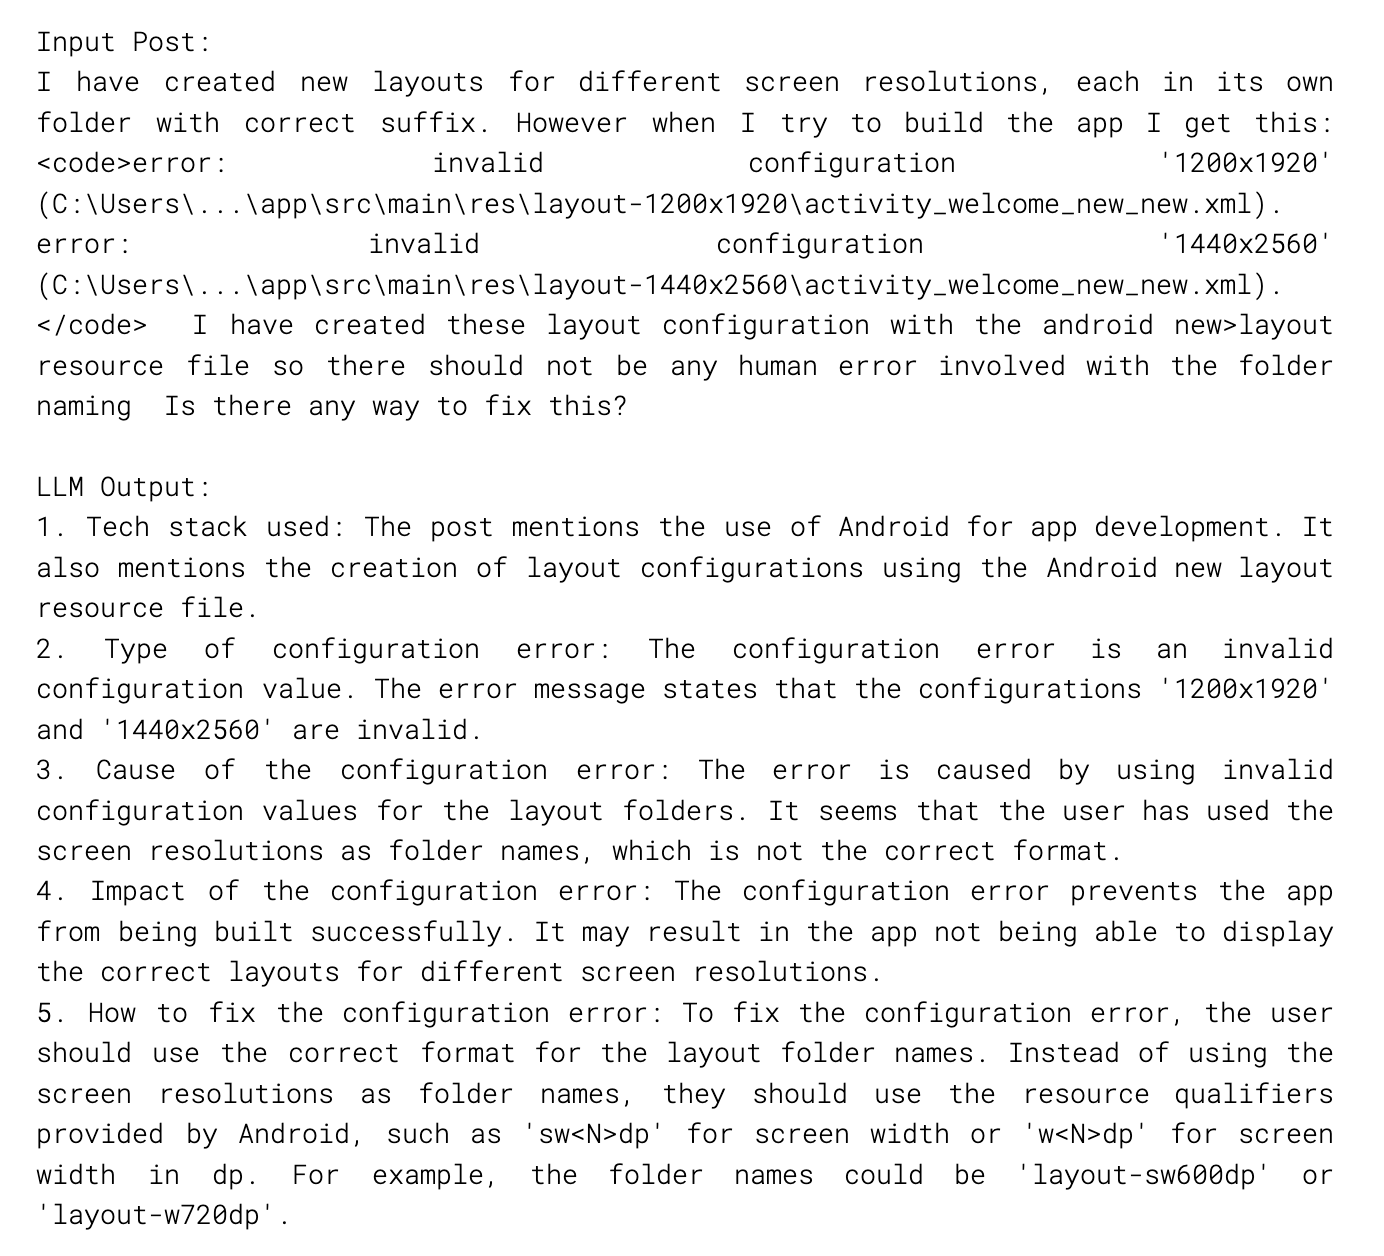
\includegraphics[width=1\textwidth]{images/analysisres.png}
  \caption{Example for LLM analyzing a SoF Post}
  \label{fig:figure512}
\end{figure}

Although specific technologies like Android Studio were not explicitly mentioned in the Tech Stack 
extraction, we deemed this categorization accurate. The error type and cause were congruent with the accepted answer for the post, showcasing the model's precision. The resolution advice provided by the LLM not only aligned with the accepted answer but also suggested the model's prior exposure to similar posts during its training phase. This may lead to inquiries about the originality of the model in generating responses. It is important to note that although the first aspect (tech stack used) did not receive a positive rating, this category consistently received high average ratings, indicating its overall reliability. The example presented in Figure \ref{fig:figure513} provides additional information on the training details of the gpt3.5-turbo model.

\begin{figure}[h]
  \centering
  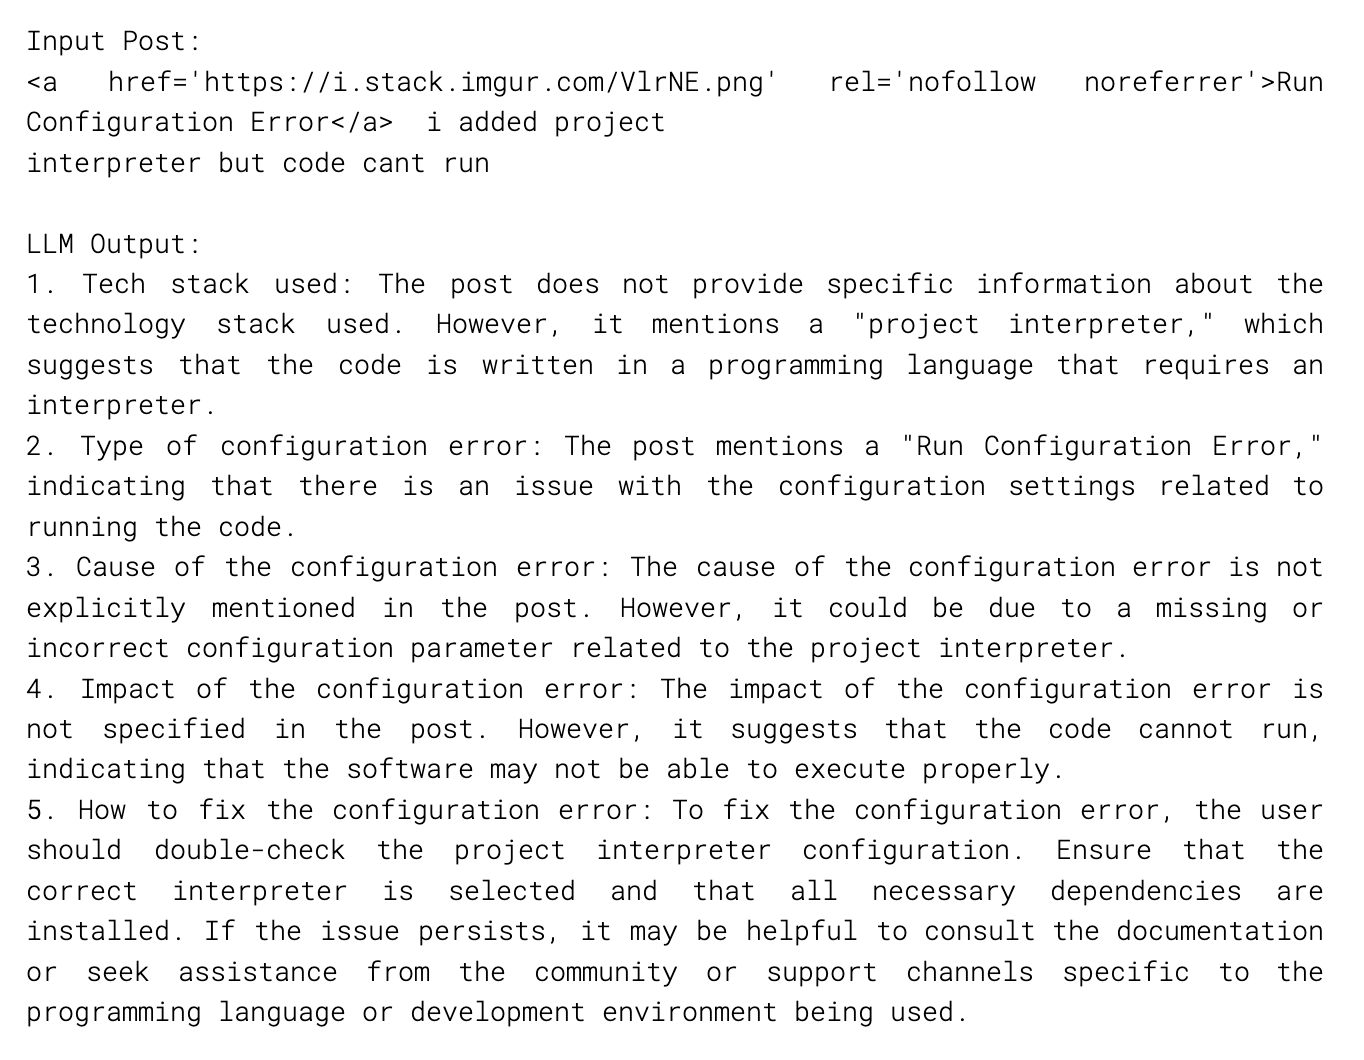
\includegraphics[width=1\textwidth]{images/failanalysis.png}
  \caption{Example for LLM attempting to analyze a SoF Post containing an image}
  \label{fig:figure513}
\end{figure}

The post's lack of specificity presents a significant challenge for the LLM, particularly since the LLM 
version used (gpt3.5-turbo) lacks image processing capabilities. The image in question displays a JetBrains PyCharm environment with a configuration window showing an error. Despite this, the model's inference about the tech stack, while speculative, aligns with our manual identification of Python and PyCharm from the image. The model's inability to precisely identify the type of configuration error from the vague description is understandable. However, its general troubleshooting guidance is creditable. This example highlights the model's limitations in scenarios involving non-textual information and emphasizes the importance of providing detailed and clear input for optimal LLM performance.

In conclusion, the experimental results provide empirical evidence that supports the effectiveness of 
the model. It demonstrates its ability to produce mostly positive and relevant responses when analyzing Stack Overflow posts related to configuration errors. This outcome not only confirms the model's usefulness in this specific domain but also suggests its potential applicability in broader technical analysis. Moving on to the next phase of our analysis results, we will now examine the specific measurements in detail. This thorough examination involves manually evaluating each output generated by the model. The assessment criterion relies on our limited knowledge in the field and is supported by the availability of accepted answers in most posts. This enables us to determine the extent to which the model aligns with established knowledge and recognized solutions within the domain of configuration errors, providing a strong framework for evaluating the model's performance.

\subsubsection{Total Result Set}

When analyzing both the set of manually labeled positive posts from the selection process and false positives classified by the LLM, the LLM demonstrated its ability to identify relevant posts without prior training. The overall score, which is detailed in Appendix 
\ref{fig:appendix3}, represents the average of positive ratings (+) given to each document, with an average score of approximately 3.21 points, or 64.2\%. The model's performance falls short of expectations for a model like gpt3.5-turbo due to the inclusion of false positives, which reduces the overall score. However, the model demonstrates improvement in datasets that only contain positively rated documents.

The LLM's average positivity ratings varied across the five analyzed aspects. The aspect of `Tech Stack Used' achieved a high average score of 0.989, demonstrating the LLM's ability to accurately identify and categorize technologies and frameworks mentioned in posts. However, there were some instances of irrelevant responses. The aspect of `Type of Configuration Error' scored 0.598, indicating difficulties in providing coherent explanations, particularly for false positives. This trend persists with the other aspects: `Cause of the Configuration Error' (0.513), `Impact of the Configuration Error' (0.602), and `How to fix the Configuration Error' (0.504). These scores demonstrate the limitations of LLM in classifying and analyzing configuration error content, particularly in identifying false positive posts, indicating areas for future model improvement.

\subsubsection{Positive Documents Result Set}

In the second variant of the analysis, which focuses on all posts we manually labeled as positive, including reclassified true positives, 9 posts that were initially considered general discussions were later recognized as relevant. The revised dataset achieved an average score of 4.559, or 91.2\%, using a 0 to 5 rating system (see Appendix 
\ref{fig:appendix4} for distribution). This performance significantly surpassed that of the first variant on the entire dataset.

In this subset, the LLM performed exceptionally well in identifying the `Tech Stack Used' with an average rating of 0.978, demonstrating its precision in recognizing technological frameworks. For `Type of Configuration Error', it achieved an average rating of 0.937, highlighting the significance of accurate initial classification. The aspect related to the `Impact of the Configuration Error' scored approximately 0.981, indicating the model's ability to comprehend both immediate and potential consequences of errors.

However, the `Cause of the Configuration Error' aspect received a slightly lower average rating of 0.841, suggesting some difficulty in identifying the sources of errors. The aspect of `How to fix the Configuration Error' received an average rating of 0.822, indicating that there is room for improvement in proposing effective solutions for identified issues.

\subsubsection{False Positives Result Set}

In the third variant, focusing on false positives identified by the few-shot prompting method, the LLM showed its ability to detect posts unrelated to configuration errors. A high average score indicates successful detection of non-error posts, while a low score suggests that the model attempts to analyze irrelevant posts. The distribution of posts across five aspects is detailed in Appendix \ref{fig:appendix5}.

The LLM achieved an average score of 1.852 for false positives, underperforming compared to other variants, with only 18.5\% of posts correctly identified as not containing configuration errors. However, in the `Tech Stack Used' category, the model excelled with an average rating of 1, accurately extracting technical details from each false positive post. However, the model exhibited significant limitations in several areas, including `Type of Configuration Failure' (0.259), `Cause of the Configuration Error' (0.185), `Impact of the Configuration Error' (0.222), and `How to fix the Configuration Error' (0.185).

These results underscore the LLM's nuanced and limited ability to identify and analyze configuration errors. Although the model accurately identifies technology stacks, its ability to understand the specifics of configuration errors, such as their types, causes, and solutions, is considerably limited. The model's difficulty in distinguishing between relevant and irrelevant content, especially in processing false positives, highlights the need for further development to improve its comprehension and analytical capabilities. The difference in findings between the positives-only set and this variant is substantial.

\chapter{Discussion}

\section{Comparison CM-PaCE \& LLM}

\subsubsection{CM-PaCE Experiment}

The initial research question of our study was to compare various machine learning approaches for 
retrieving Stack Overflow posts about configuration errors. This question was addressed in the first two experiments. Initially, we developed our own classification model, CM-PaCE, which performed well in classifying our manually selected dataset. Based on the results and experience gained from the experiment, it can be confidently stated that training classification models specific to a certain domain of knowledge, such as retrieving posts from Stack Overflow, can be particularly helpful. Although there were initial concerns about the Word2Vec model's ability to comprehend technical domain configuration errors, our study found that the model produced satisfactory results even with a relatively small dataset. However, it is important to note that such a dataset must be collected and curated beforehand.

When considering the work of \citet{tian:2020}, it is evident that the authors' proposed 
combination of Word2Vec and SVM yielded favorable results. Additionally, their findings suggest the utilization of classification models for the automated retrieval of a substantial dataset of posts from Stack Overflow. Although their domain of Architecture Smells differs from our task of retrieving posts discussing Configuration Errors, we are pleased to see that the results and implications have similar outcomes in highlighting the capabilities of such models.

\subsubsection{LLM Experiment}

In the second experiment, we tested an LLM using the gpt3.5-turbo model by OpenAI to answer the 
research question. The results were thoroughly positive. When comparing different prompting methods, we found that the Few-Shot prompting method yielded the best results. This hybrid approach improves the quality of classifications and demonstrates the potential of combining systematic LLM methodologies with targeted criteria from manual processes. The method shows promise for automated classification tasks, especially in the technical content analysis domain. The use of LLMs represents progress in utilizing their capabilities for accurate and dependable automated analysis, a crucial development in the field of AI-driven data classification.

One major limitation observed in the second experiment across all four prompting methods was the 
incidence of false positives. Although some posts were later reclassified as containing talk about configuration errors, the model misclassified some posts as false positives and failed to recognize others as not containing configuration errors in the analysis experiment. This could be caused by the presence of hallucinations, which is still a major topic for LLMs. However, it could also be due to the fact that the general topic of configuration was sufficient for the model to classify it as containing talk about configuration errors.

Additionally, the deployment of the LLM, trained on an extensive dataset, demonstrated its proficiency 
in text generation, providing further insights into the model's reasoning processes. This capability extends beyond the primary task of merely classifying posts, offering valuable perspectives on the broader competencies of LLMs. The model's ability to generate coherent and contextually relevant text highlights its potential not only in categorizing content but also in enhancing our understanding of complex subjects. This feature is especially useful in domains where contextual understanding and explanatory depth are crucial, further establishing the role of LLMs in advanced data analysis and interpretation. Exploring this aspect of the LLM's functionality suggests its usefulness in various applications, from automated content creation to assisting in sophisticated analytical tasks, thus expanding the scope of AI applications in data-driven research and development.

\subsubsection{Comparison}

The comparison between the CM-PaCE model, which combines Word2Vec and SVM and operates locally, and 
large language models (LLMs) for classifying Stack Overflow posts about configuration errors, aims to answer some questions. First, what are the use cases for a localized model such as CM-PaCE? The CM-PaCE model is tailored for specific tasks, offering enhanced performance with potentially lower computational demands. This makes it a suitable choice for applications with limited computational resources or requiring high customization to address specific configuration errors. However, its effectiveness is closely tied to hyperparameter optimization and the breadth of the training dataset. Improving these aspects could significantly enhance its performance, demonstrating the potential of specialized models in domain-specific classification tasks.

Next, when does it make sense to utilize LLMs for a classification task? LLMs, with their extensive training on diverse datasets, offer a level of 
versatility and depth that is difficult to match with more specialized models. This breadth of knowledge allows them to provide comprehensive analysis across various domains and contexts, which is critical when dealing with the multifaceted nature of configuration errors. Additionally, their ability to provide explanations for classification decisions further enhances their analytical utility. LLMs require higher computational resources and may not be as efficient as localized models like CM-PaCE in terms of speed. However, their out-of-the-box readiness and adaptability make them a compelling choice for broader, more comprehensive analytical tasks. This trade-off between specialized efficiency and versatile depth is a key consideration when selecting the appropriate model for classifying and analyzing configuration errors in different scenarios.

When addressing the first research question, `\textbf{How do different Machine 
Learning Approaches compare to retrieve Stack Overflow posts about configuration errors?}', our findings reveal a nuanced landscape. The CM-PaCE model demonstrates proficiency in targeted retrieval, benefiting from its tailored design to precisely identify configuration error-related posts with lower computational overhead. In contrast, LLMs exhibit remarkable versatility and depth due to their extensive training across a wide array of datasets. However, this comes at the cost of increased computational demands.

\section{Analysis of Configuration Errors using LLM}

For the third experiment, it is useful to ask if LLMs are well-suited for the analysis of data. Utilizing the LLM gpt3.5-turbo from OpenAI we aimed to analyze a dataset of Stack Overflow 
posts and evaluate the LLMs performance. The analysis focused on five aspects: `Tech Stack Used', `Type of Configuration Error', `Cause of the Configuration Error', `Impact of the Configuration Error', and `How to Fix the Configuration Error'. The LLM demonstrated superior performance on a subset of posts that were manually identified as relevant to configuration errors. Notably, it excelled in identifying the `Tech Stack Used'. The model's proficiency can be attributed to its extensive training on diverse technological contexts, enabling it to accurately recognize and categorize various tech stacks. This finding suggests that LLMs, with their vast exposure to technical data, can become effective tools in rapidly identifying the technological environment of a given problem, which is crucial for prompt and accurate error resolution.

The analysis yielded positive results for the set of posts that were manually labeled as positive during the dataset collection process. However, the analysis of the dataset containing both our positive labeled posts and the false negatives produced by the model, and the set comprising only false positives was less effective, highlighting the importance of accurate pre-classification of posts. The Few-Shot prompting method was the most effective because it engages the LLM to pre-train on some examples, improving the reasoning process. This method was instrumental in filtering relevant data from irrelevant data, thereby enhancing the overall accuracy of the analysis.

One interesting question when talking about the analysis is, did the model exhibited limitations in logical reasoning? This was indeed the case for a small but noteworthy amount of posts. For instance, it correctly identified Maven in 
the `Tech Stack Used' section but failed to deduce that Java was the associated programming language. This discrepancy highlights the need for more sophisticated and directive prompting techniques to improve the model's inferential reasoning abilities. The limitations of the LLM in processing indirect or less common information are accentuated by its optimal performance with familiar solutions and common errors. This suggests a need for more sophisticated models capable of nuanced understanding and reasoning.

In conclusion, the LLM demonstrated proficiency in extracting information about configuration errors, 
primarily with the set of relevant documents. However, our limited domain expertise restricted a comprehensive interpretation of the results. Nonetheless, the consistency observed in the results provides a promising foundation for future, more in-depth investigations of configuration errors, their interrelationships across different technology stacks, and their impact. Regarding the research question `\textbf{How do LLMs help to analyze retrieved datasets?}', we can confidently assert that LLMs significantly aid in the automated extraction of information from large amounts of data. This claim is supported by comparing the model outputs with the accepted answers on Stack Overflow, showing a high level of agreement between the model's findings and the community-validated solutions.

\section{Potential Applications of our Method}

Large language models have great potential for advancing research on configuration errors. They 
can automate post classification and extract useful information about configuration errors. This functionality enables various applications, including automated dataset creation and aiding in the analysis of information extracted from posts, not limited to configuration errors but encompassing other technical subjects as well. However, it is important to acknowledge the challenges encountered, such as the prevalence of false positives and instances of hallucination. Improving these issues can be achieved by enhancing prompting methodologies, refining training data, or adopting more advanced LLMs.

Additionally, our research highlights the effectiveness of creating customized, concise classification 
models for the task, such as our CM-PaCE model. With the work of \citet{tian:2020} and our classification task we can confidently state that the potential for such tools exists, even with relatively small datasets for a tech-specific domain. A specialized classification model could be employed to isolate relevant documents, which could subsequently be analyzed by an LLM to discern the technical domain in question, combining both a traditional machine learning approach with the abilities of large language models.

The comparison of different prompting methods provided valuable insights into the operational dynamics 
of LLMs and the optimal strategies for their application in highly specialized technical domains like ours. The examination offers a nuanced understanding of the complexities and variances inherent in different prompting techniques for LLMs, particularly in tasks like ours. Our research findings could assist developers in devising new techniques for extracting documents from large datasets. Additionally, researchers could benefit from our insights into document analysis using LLMs. However, it is important to exercise caution due to the potential for hallucinations in these models.

\section{Threats to Validity}

\subsubsection{Dataset Creation}

There are limitations resulting from the manual data collection. One major limitation is the potential for bias introduced by the author conducting the data collection alone. In contrast, \citet{tian:2020} had two authors manually collect and discuss posts, with a third author resolving disagreements. In this work, posts were collected based on predetermined criteria with no guarantee against unconscious bias. For instance, some posts may be misclassified as false when they are actually related to configuration errors. This is the case for 9 documents as we further analyzed the dataset during the third experiment. The updated documents we misclassified are only taken into account into the third experiment as we already conducted the first two experiments. To mitigate these issues, we carefully designed our criteria according to not only the work of \citet{tian:2020} but also the general aspects of configuration errors from further research.

The dataset size presents another challenge. To address this, we utilized the work of \citet{tian:2020}, who collected a total of 395 posts. We aimed to increase the dataset by 50\% to ensure sufficient data. However, in real-world applications, models are frequently trained on millions of documents. 

\subsubsection{Word2Vec \& SVM Libraries}

When developing models that use external libraries, such as gensim's Word2Vec and scikit-learn's SVM for Python, it is important to acknowledge any potential limitations inherent to these tools. Although these libraries are widely used and have been thoroughly tested within the community, it is still necessary to consider that they may introduce specific issues or biases. However, despite their widespread adoption and rigorous validation, it is unlikely that these libraries significantly compromise the integrity or accuracy of our model. Nevertheless, we must carefully consider this aspect to ensure the robustness and validity of our model.

\subsubsection{Large Language Model}

During the evaluation process, a major issue arose regarding the maximum length that the model's API 
could handle. Two documents were excluded from the Few-Shot prompting method due to the extended initial prompt, which included four examples combined with two large posts, exceeding the maximum character limit for the model. However, we included these two documents in the other methods since we had already evaluated the first method with them. Repeating the entire experiment from this point was not feasible due to the limited token budget.

Additionally, the prompts themselves may be faulty. Although we constructed the prompts after testing 
with different versions, we could not cover the full potential of the LLM. There may be more specific prompts that perform better than ours, even though we used the most common prompting methods. However, based on the initial testing we conducted, we believe that our prompts are suitable for the task at hand. To address this issue, we suggest testing different prompts or comparing our evaluation of the full dataset with evaluations from other prompts to identify areas for improvement.

Another major consideration is that the model we used for our experiment, gpt3.5-turbo by OpenAI, is 
subject to constant changes. The version we used was gpt-3.5-turbo-0613. Newer versions may significantly alter results due to improvements in semantic stability, domain knowledge, and context. Large language models have undergone significant changes in a short time, and future models may outperform the one used in this study. This presents an opportunity for future research to compare different LLM models over time and measure their results against ours.

Finally, a significant issue with LLMs, such as gpt3.5-turbo, is the risk of hallucination. As explained 
earlier, LLMs can generate additional information that does not reflect reality in their attempt to produce an output. In our experiment, we aimed to reduce the risk of hallucination by lowering the model's temperature parameter. However, this issue is still prominent when the model is presented with severe logical conclusions, as in the analysis experiment. This could lead to severe problems during classification if the prompts are not thoroughly evaluated before applying this approach.

Another limitation that is present with LLMs is the uncertainty of prior training on documents from our dataset. The model may have been trained on millions of posts from Stack Overflow, including posts from our dataset, therefore making it unclear whether the dataset really included `new documents' for the model. 

\section{Future Research}

Future research for this study is diverse and accessible. One area of improvement is the optimization 
of developing a specialized classification model. Specifically, starting with CM-PaCE, there are numerous configuration options in the hyperparameters and dataset that can significantly enhance the model's performance, potentially surpassing even future LLMs. Additionally, increasing the dataset size can further improve the model's ability to comprehend technical details in these domains. Utilizing Natural Language Processing abilities for such models opens up new areas. 

The model may be able to improve the classification process, provide useful information, or analyze documents in ways that were previously only possible with third-party LLMs. Developing a specialized NLP model for highly technical fields offers a great way to automate tasks in research and development. Further utizlizing the capabilities of LLMs can be achieved by fine-tuning an LLM in the tech-specific field of configuration errors.

Finally, the dataset can be enriched with additional information that can be used when working with LLMs, such as the accepted answer, tags, or other metadata. Our focus was only on the main content of the posts, but there are many more possibilities that can be explored. Additionally, the fine-tuning of LLMs can potentially yield thorough positive results by utilizing a smaller model that is trained for a tech-specific task.

\chapter{Conclusion}

The growing complexity of software systems and their susceptibility to configuration errors highlights the critical need for effective resolution methods. Configuration errors can have significant consequences, ranging from system downtime to severe security risks. These errors often result from human error or a lack of system familiarity. It is important to avoid such errors by ensuring proper training and familiarity with the system. The 2021 Meta outage is a striking example of this, resulting in substantial financial loss and emphasizing the urgent need for improved management of configuration errors (\citet{guardian:2021}).

To tackle this problem, we conducted research that utilized posts from Stack Overflow, which is a crucial resource for developers who face configuration challenges. Our approach consisted of two complementary methodologies. First, we developed a machine learning model that was trained to identify patterns in discussions about configuration errors on Stack Overflow. This model used Word2Vec for feature extraction and SVM for classification. Second, we investigated the use of large language models (LLMs), such as GPT-3.5, for similar purposes. The LLMs were expected to provide coherent and contextually relevant responses, thereby facilitating the categorization and analysis of posts related to configuration errors.

The findings suggest that both approaches hold potential for addressing the problem. Our CM-PaCE model demonstrated the ability to accurately identify relevant posts, validating the effectiveness of Word2Vec and SVM in classifying configuration errors. The approach based on LLM and leveraging GPT-3.5 also demonstrated significant potential. It was particularly adept at handling varying levels of user expertise and generating contextually coherent responses, thus enhancing the efficiency and depth of analysis. These findings indicate a strong potential for fine-tuning such models and using them in other technology-related fields.

In conclusion, our research contributes to the growing field of automated configuration error identification and analysis. We successfully applied machine learning and LLMs to real-world data from Stack Overflow, offering insights and methodologies for tackling the complex issue of configuration errors. The integration of these approaches can aid developers and system administrators in preempting and resolving configuration-related challenges, leading to more robust and reliable software systems. Further research could explore the scalability of these methods and their adaptability to other types of software errors, paving the way for broader applications in software maintenance and development.

% Appendix
\appendix

\chapter{Methodology Appendix}

\begin{figure}[h]
  \begin{tcolorbox}[enhanced jigsaw,drop shadow=black!50!white,colback=white]
    The following input is a post from Stack Overflow. Your task is to classify if the post contains configuration errors or talk about it.\\
The post may contain the following information:\\
- A topic that mentions configuration errors, this can be the user talking about configurations and resulting errors, or an error reported by the user which can be the result of a configuration error.\\
- Code that implies configuration errors, either by the user directly stating the error or your knowledge on configuration errors for a given code section. Code sections in the input are marked with <code>\\
Keep in mind that the post is raw text and contains various html tags indicating different parts of the post, such as headings or code sections.\\
If the post contains configuration errors or talk about configuration errors, reply with `yes' and include a short explanation for your decision, such as the possible configuration error.\\
If the post does not contain configuration errors or talk about configuration errors, reply with `no' and include a short explanation for your decision, for example if the post is about configurations, but not specifically about configuration errors.
  \end{tcolorbox}
  \caption{Zero-Shot prompting prompt}
  \label{fig:figure45}
\end{figure}

\begin{figure}[h]
  \begin{tcolorbox}[enhanced jigsaw,drop shadow=black!50!white,colback=white]
    The following input is a post from Stack Overflow. Your task is to classify if the post contains configuration errors or talk about it.\\
The post may contain the following information:\\
- A topic that mentions configuration errors, this can be the user talking about configurations and resulting errors, or an error reported by the user which can be the result of a configuration error.\\
- Code that implies configuration errors, either by the user directly stating the error or your knowledge on configuration errors for a given code section. Code sections in the input are marked with <code>\\
Keep in mind that the post is raw text and contains various html tags indicating different parts of the post, such as headings or code sections.\\
Here are two examples of Stack Overflow posts that contain configuration errors:\\
\lbrack Example 1\rbrack\\
\lbrack Example 2\rbrack\\
And here are two examples of Stack Overflow posts that do not contain configuration errors:\\
\lbrack Example 1\rbrack\\
\lbrack Example 2\rbrack\\
If the post contains configuration errors or talk about configuration errors, reply with `yes' and include a short explanation for your decision, such as the possible configuration error.\\
If the post does not contain configuration errors or talk about configuration errors, reply with `no' and include a short explanation for your decision, for example if the post is about configurations, but not specifically about configuration errors.
  \end{tcolorbox}
  \caption{Few-Shot prompting prompt}
  \label{fig:figure46}
\end{figure}

\begin{figure}[h]
  \begin{tcolorbox}[enhanced jigsaw,drop shadow=black!50!white,colback=white]
    The following input is a post from Stack Overflow. Your task is to classify if the post contains configuration errors or talk about it.\\
  The post may contain the following information:\\
  - A topic that mentions configuration errors, this can be the user talking about configurations and resulting errors, or an error reported by the user which can be the result of a configuration error.\\
  - Code that implies configuration errors, either by the user directly stating the error or your knowledge on configuration errors for a given code section. Code sections in the input are marked with <code>\\
  Keep in mind that the post is raw text and contains various html tags indicating different parts of the post, such as headings or code sections.\\
  If the post contains configuration errors or talk about configuration errors, reply with `yes' and include a short explanation for your decision, such as the possible configuration error.\\
  If the post does not contain configuration errors or talk about configuration errors, reply with `no' and include a short explanation for your decision, for example if the post is about configurations, but not specifically about configuration errors.\\
  Following the input, let's think step by step on how to find the best solution.
  \end{tcolorbox}
  \caption{Chain-of-Thought prompting prompt}
  \label{fig:figure47}
\end{figure}

\begin{figure}[h]
  \begin{tcolorbox}[enhanced jigsaw,drop shadow=black!50!white,colback=white]
    The following input is a post from Stack Overflow. Your task is to classify if the post contains configuration errors or talk about it.\\
The post may satisfy the following criteria that indicate if configuration errors are present or if the user has a problem that indicates
configuration errors:\\
- The description of a configuration error by the user\\
- Description of causes that lead to a configuration error\\
- Methods used to detect/refactor specific configuration errors\\
- Discussion about tools for detecting and resolving specific configuration errors\\
- Discussion about the impact of a configuration error on software development\\
- Challenges identified in detecting and resolving configuration errors\\
Use these criteria to classify the post.\\
If at least one of these criteria is true, reply with `yes' and include a short explanation for your decision, such as the possible configuration error.\\
If non of these criteria is true, for example if the post is about configuration but not configuration errors, or the post is about a completely different topic, reply with `no' and include a short explanation for your decision, for example if the post is about configurations, but not specifically about configuration errors.\\
Keep in mind that the post is raw text and contains various html tags indicating different parts of the post, such as headings or code sections.\\
Following the input, let's think step by step on how to find the best solution using the given criteria.
  \end{tcolorbox}
  \caption{Extended Chain-of-Thought prompting prompt}
  \label{fig:figure48}
\end{figure}

\chapter{Results Appendix}

\begin{figure}[h]
  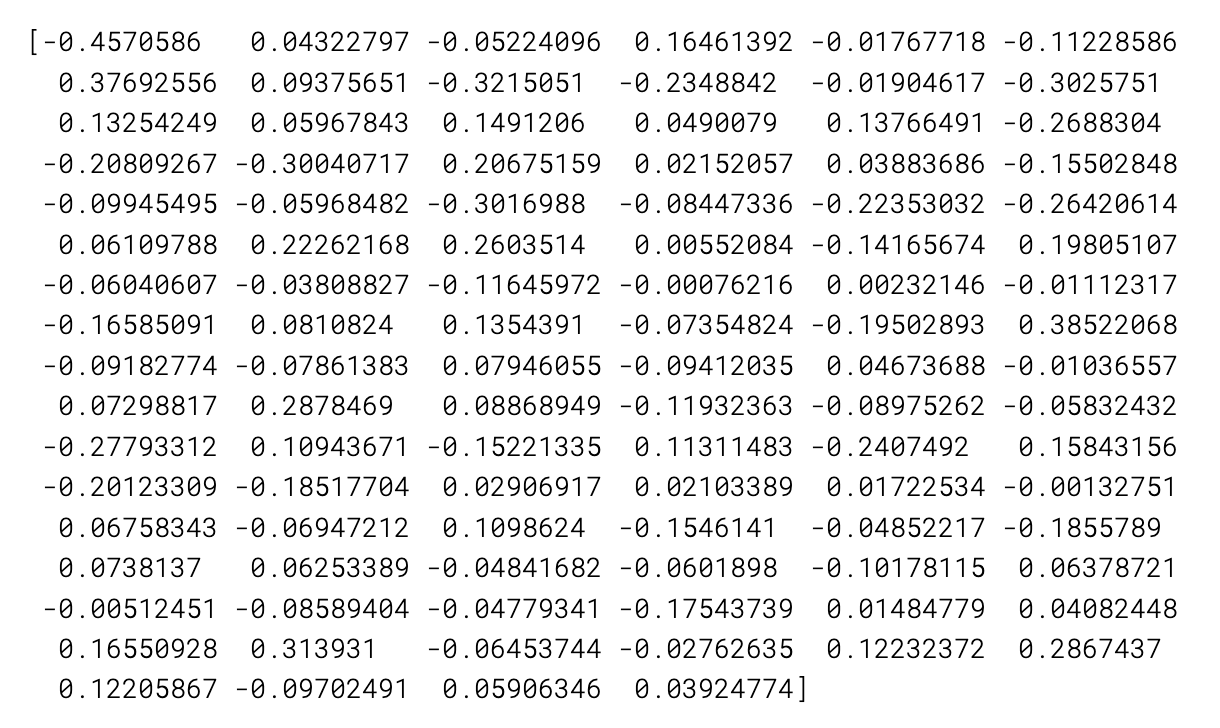
\includegraphics[width=1\textwidth]{images/featvector.png}
  \caption{Feature Vector for `configur'}
  \label{fig:figure51}
\end{figure}

\begin{figure}[h]
  \centering
  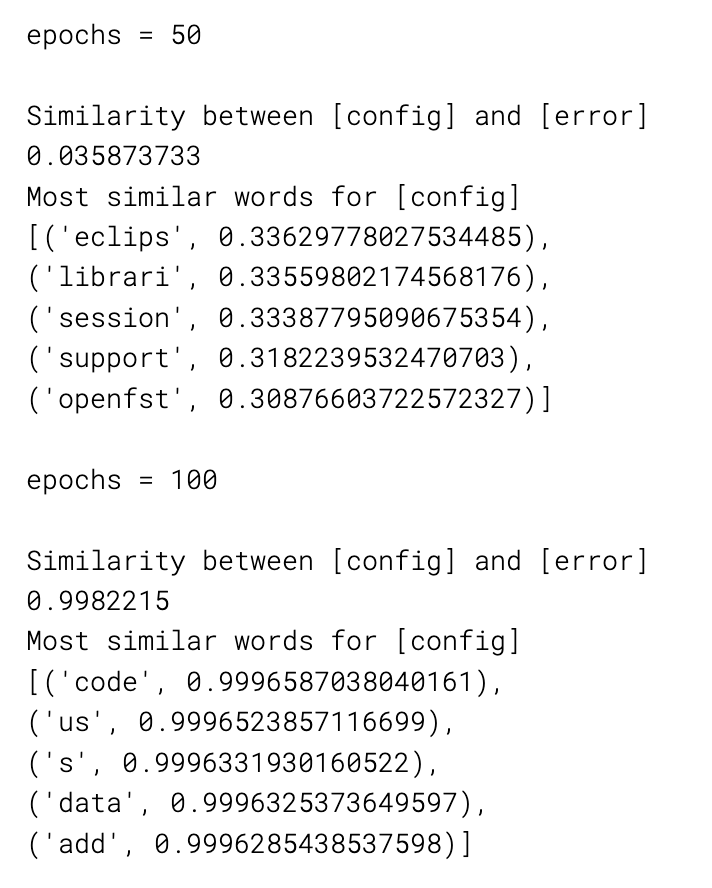
\includegraphics[width=0.65\textwidth]{images/epochres.png}
  \caption{Similarity and Similar Word results for different epochs values}
  \label{fig:figure54}
\end{figure}

\begin{figure}[h]
  \centering
  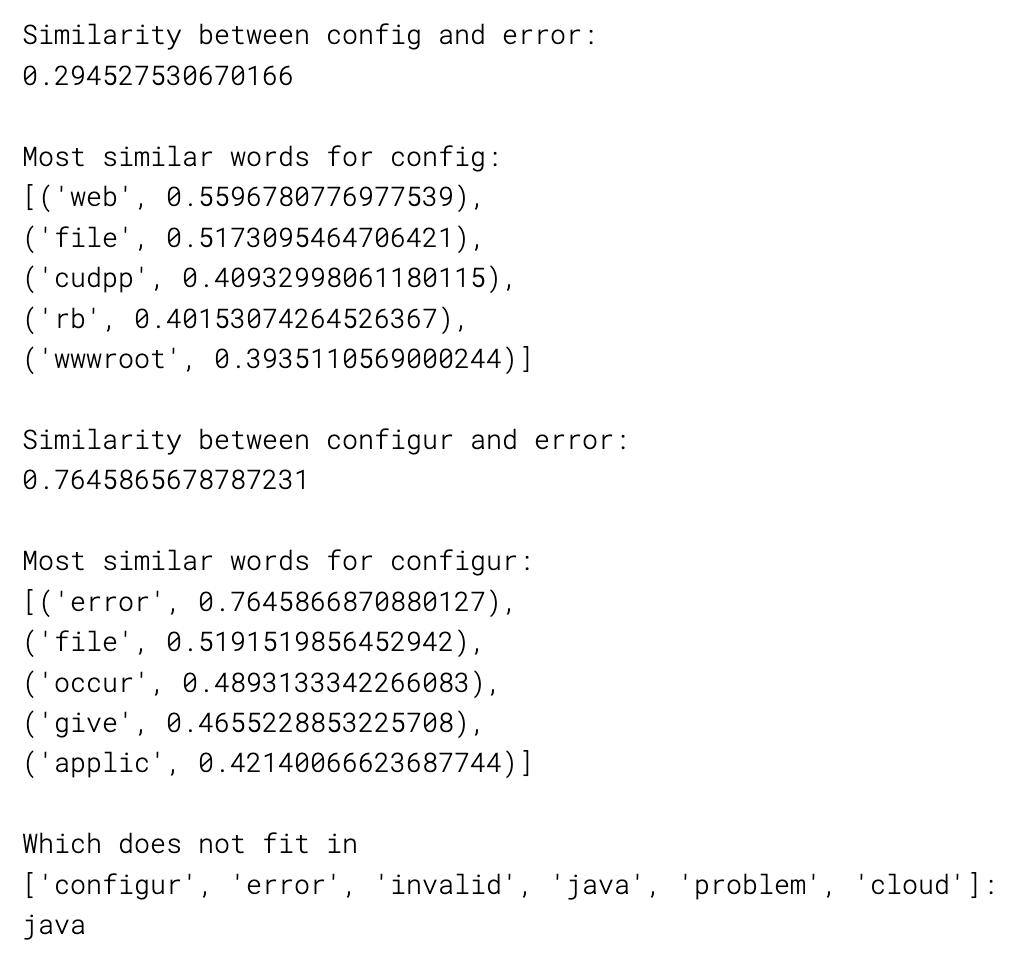
\includegraphics[width=0.9\textwidth]{images/bestword2vec.png}
  \caption{Results for best performing hyperparameter configuration}
  \label{fig:figure56}
\end{figure}

\begin{figure}[h]
  \centering
  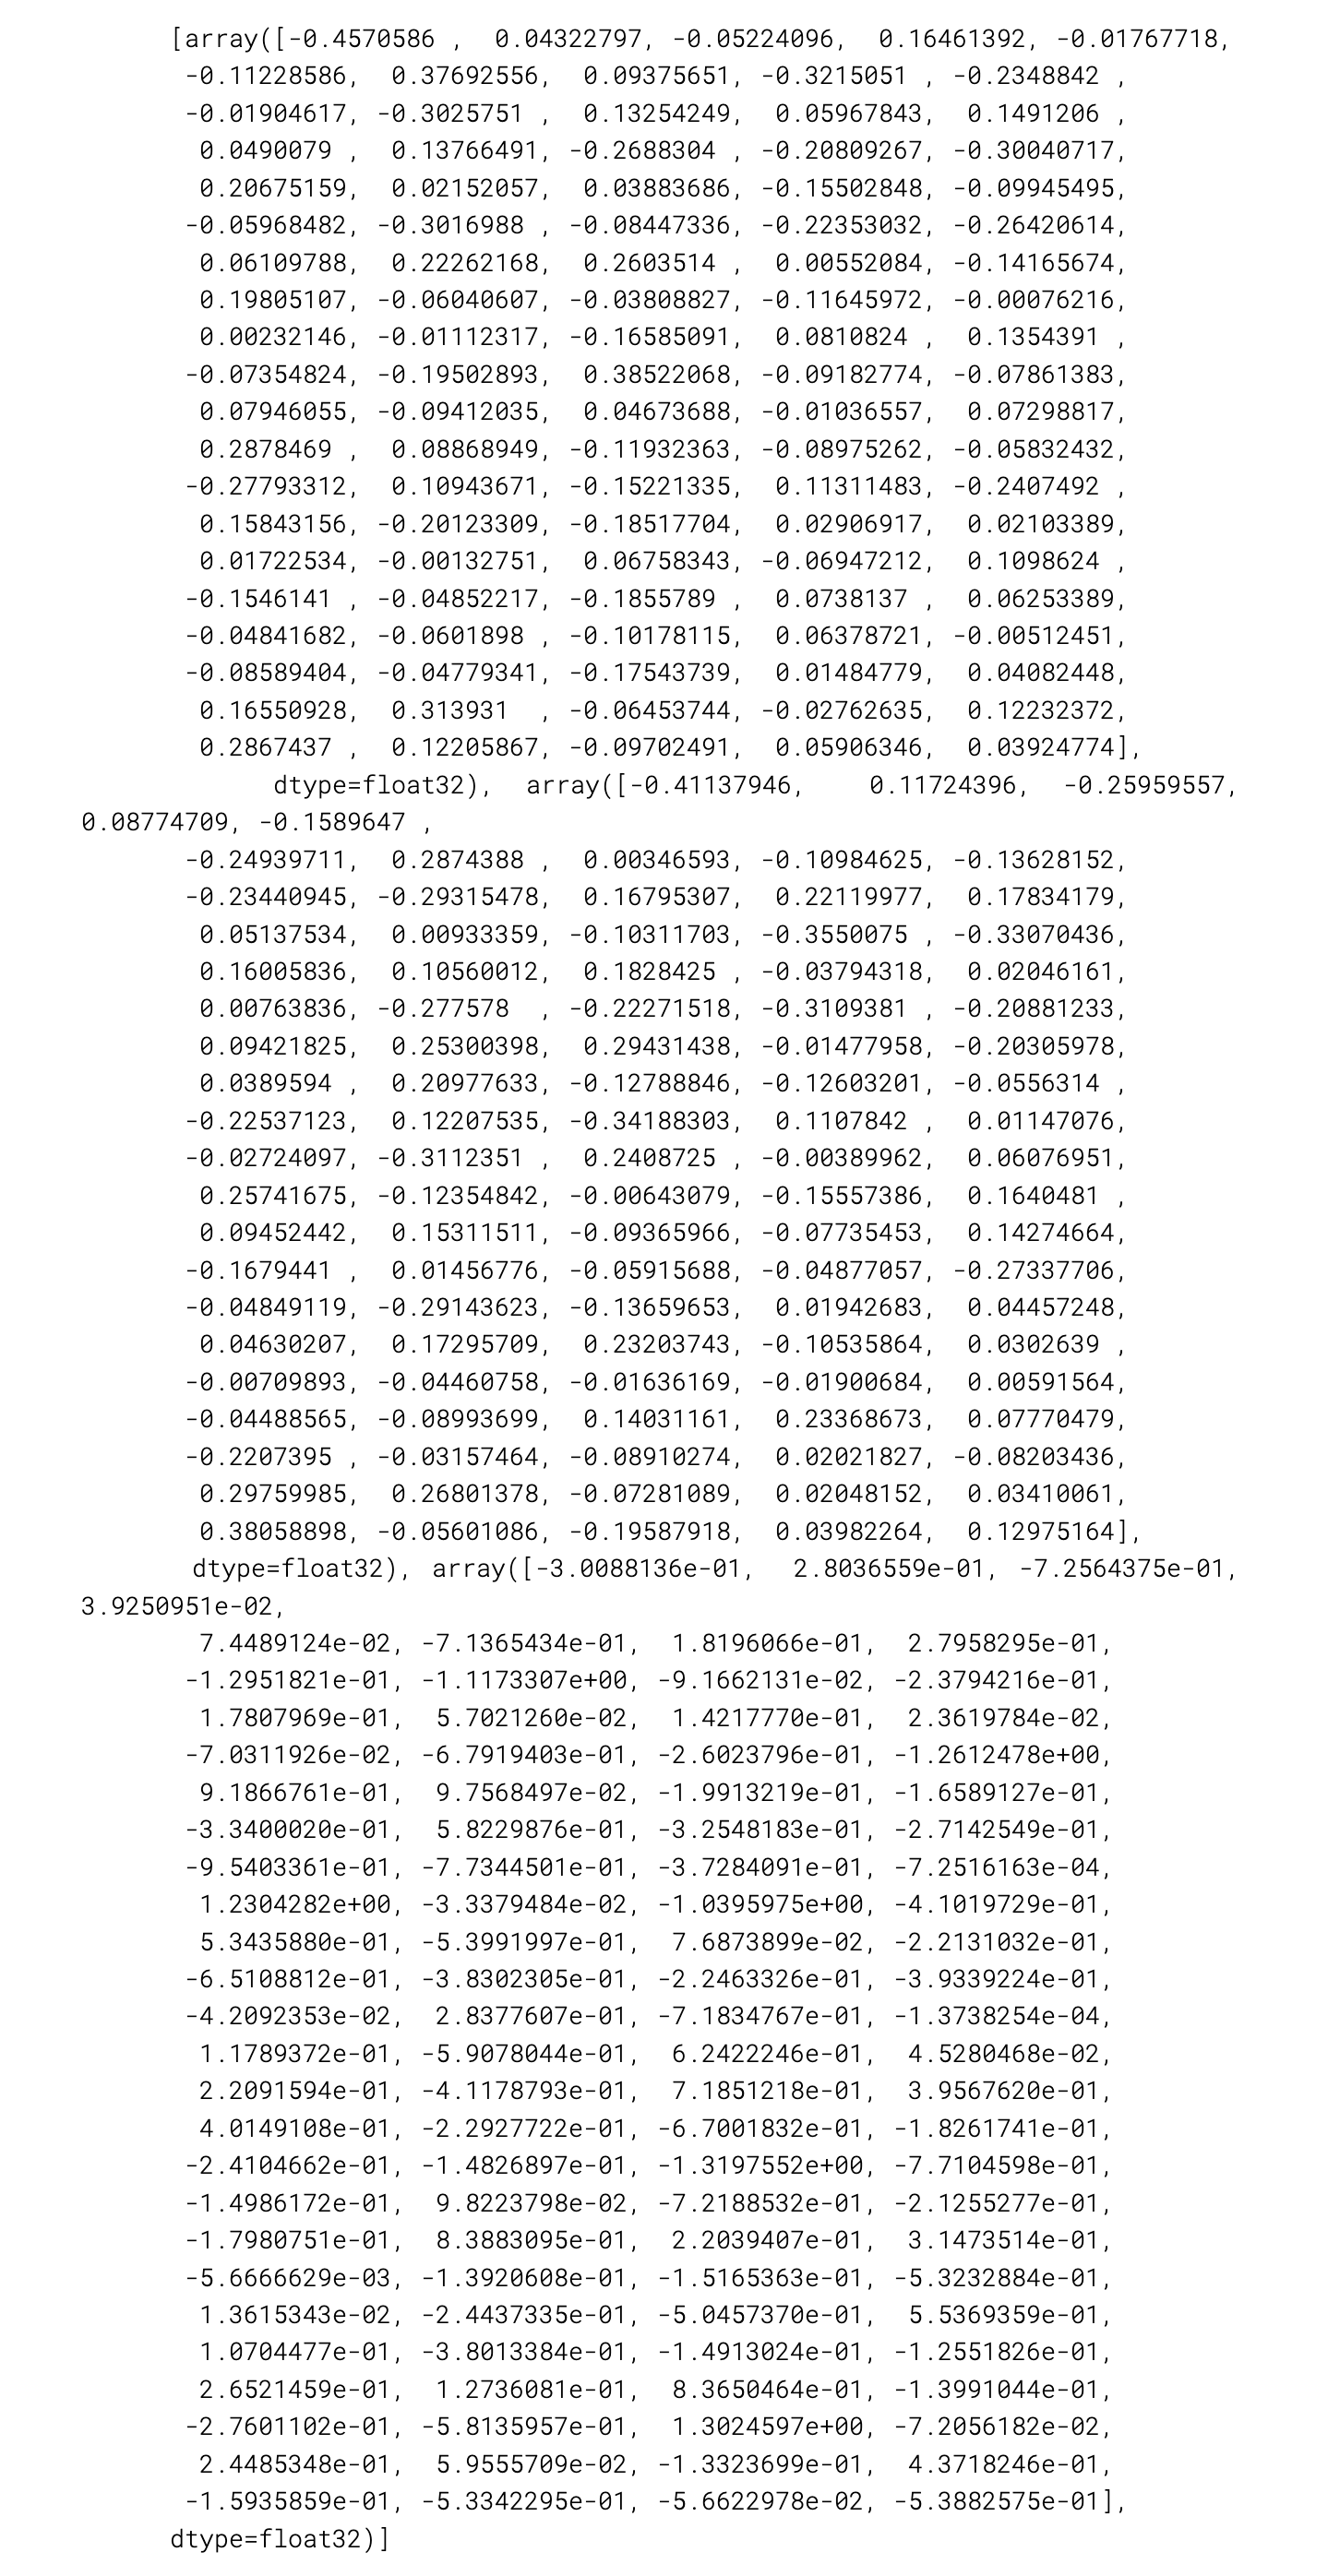
\includegraphics[width=0.7\textwidth]{images/sentence.png}
  \caption{Feature Vectors for a tokenized sentence}
  \label{fig:appendix1}
\end{figure}

\begin{figure}[h]
  \centering
  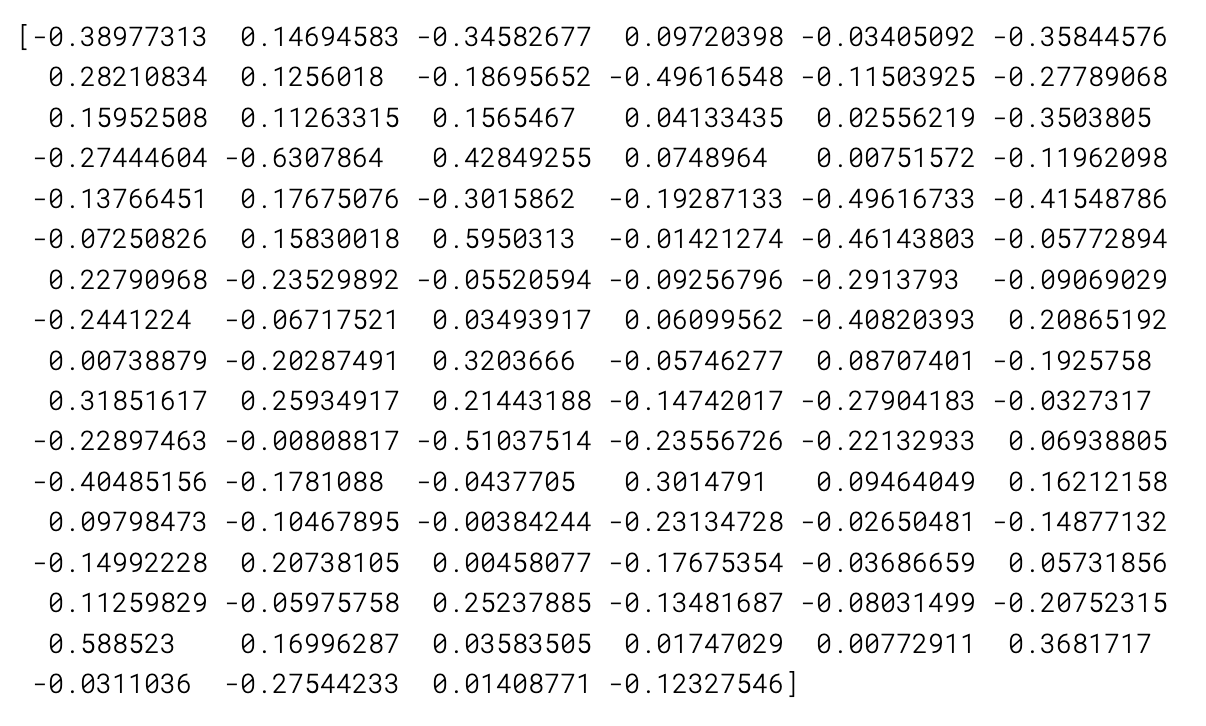
\includegraphics[width=1\textwidth]{images/vecsentence.png}
  \caption{Aggregated sentence vector}
  \label{fig:appendix2}
\end{figure}

\begin{figure}[h]
  \centering
  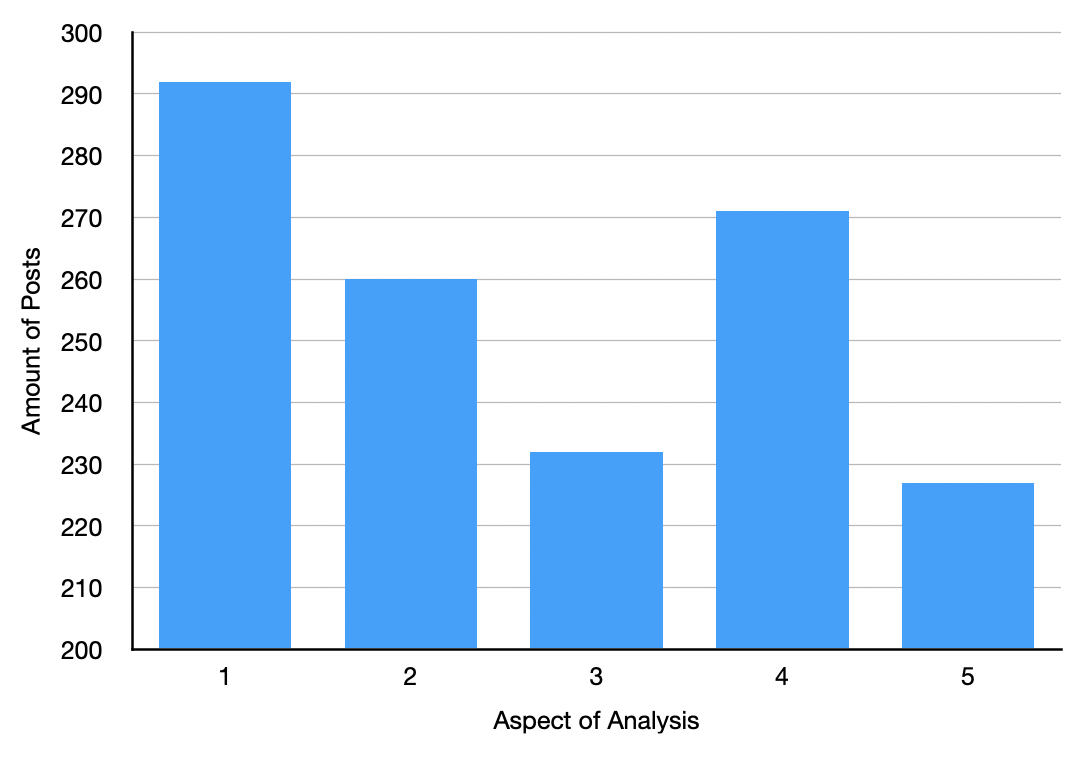
\includegraphics[width=1\textwidth]{images/table_setA.png}
  \caption{Distribution of posts on the five aspects of analysis for the total dataset}
  \label{fig:appendix3}
\end{figure}

\begin{figure}[h]
  \centering
  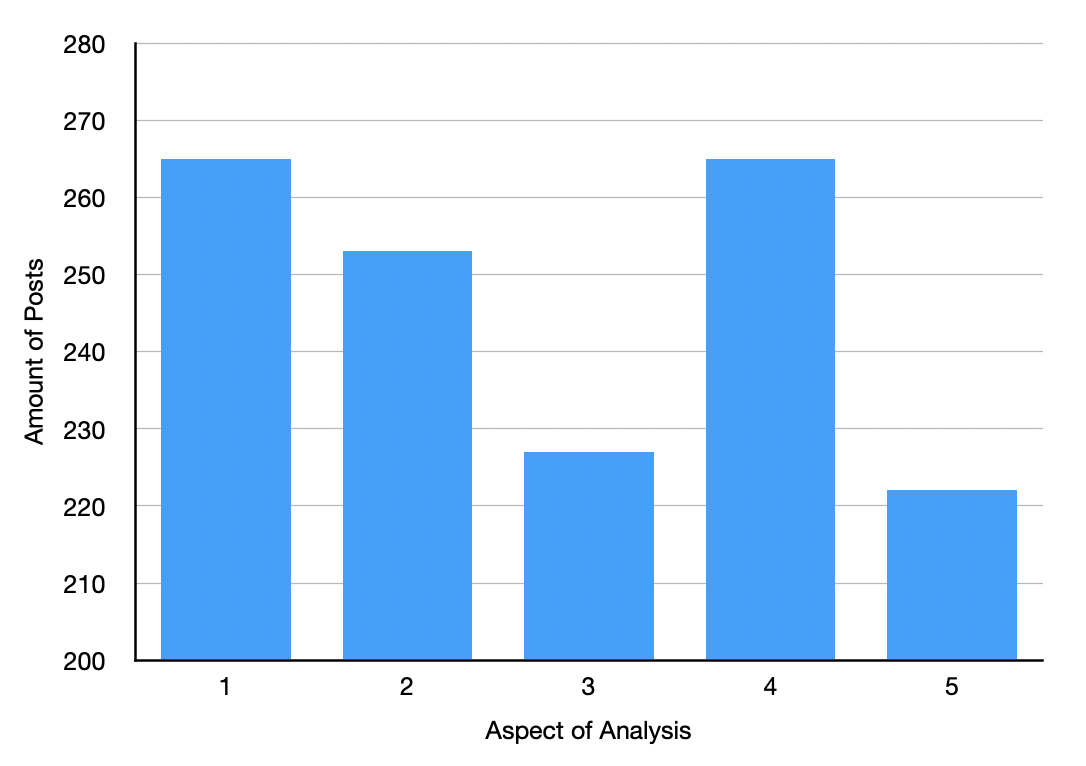
\includegraphics[width=1\textwidth]{images/table_setB.png}
  \caption{Distribution of posts on the five aspects of analysis for the set of positive documents}
  \label{fig:appendix4}
\end{figure}

\begin{figure}[h]
  \centering
  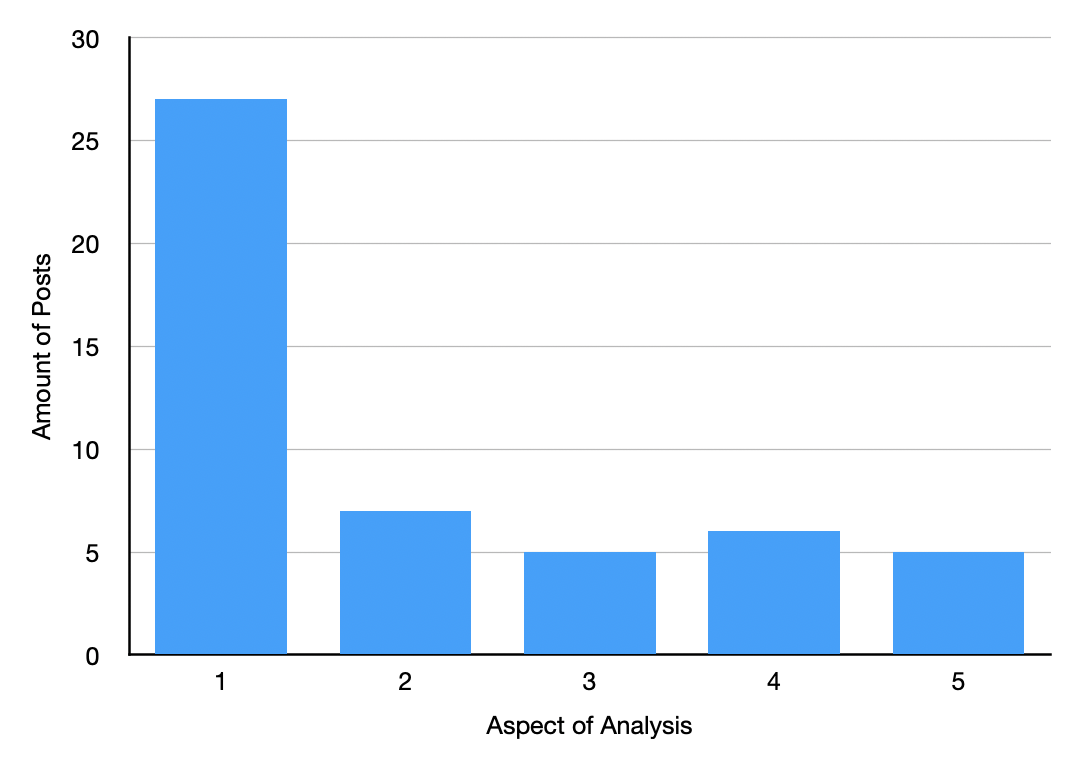
\includegraphics[width=1\textwidth]{images/table_setC.png}
  \caption{Distribution of posts on the five aspects of analysis for false positives}
  \label{fig:appendix5}
\end{figure}

% Bibliography
\bibliographystyle{plainnat} % requires package natbib. An alternative is apalike
\bibliography{literature}    % load file literature.bib

\end{document}